\documentclass{article}
\usepackage{iclr2018_conference, times}
\usepackage{hyperref}       % hyperlinks
\usepackage{url}            % simple URL typesetting
\usepackage{booktabs}       % professional-quality tables
\usepackage{amsfonts}       % blackboard math symbols
\usepackage{nicefrac}       % compact symbols for 1/2, etc.
\usepackage{microtype}      % microtypography
\usepackage{amsmath}
\usepackage{amsthm}
\usepackage{hyperref}
\usepackage{graphicx}
\usepackage{algorithm}
\usepackage{algpseudocode}
\usepackage{algorithm}
\usepackage{subcaption}
\usepackage{algpseudocode}
\usepackage{wrapfig} % for side-by
\usepackage{bm}
% rename algorithmic labels
\renewcommand{\algorithmicensure}{\textbf{return}}
\renewcommand{\algorithmicfunction}{\textbf{def}}

\definecolor{mydarkblue}{rgb}{0,0.08,0.45}
\hypersetup{colorlinks=true,
    linkcolor=mydarkblue,
    citecolor=mydarkblue,
    filecolor=mydarkblue,
    urlcolor=mydarkblue}

\newcommand{\vtheta}{\mathbf{\theta}}
\newcommand{\relaxed}{r}
\newcommand{\controlf}{c}  % Control variate for functions
\newcommand{\controlg}{\hat g}  % Control variate for gradients
\newcommand{\discreteDist}{p(b|\theta)}
\newcommand{\loss}{f(b)}
\newcommand{\lossGrad}{\loss{} \frac{\partial}{\partial \theta }\log \discreteDist{}}
\newcommand{\mcGrad}{\hat{g}}
\newcommand{\expectedLoss}{\mathbb{E}_{\discreteDist{}} \! \left[ \, \loss{} \right]}
\newcommand{\expectedLossLogTrick}{\mathbb{E}_{\discreteDist{}} \! \left[ \, \lossGrad{} \right]}
\newcommand{\var}{\mathbb{V}}
\newcommand{\vu}{\mathbf{u}}
\newcommand{\E}{\mathbb{E}}
\newcommand{\LL}[1]{\frac{\partial \log \pi(a_{#1}| s_{#1}, \theta)}{\partial \theta}}
\newcommand{\PT}{\frac{\partial}{\partial \theta}}
\newcommand{\PP}[1]{\frac{\partial}{\partial #1}}
\newcommand{\PPH}{\frac{\partial}{\partial \phi}}
\newcommand{\LP}[1]{\PT \log p(#1)}
\newcommand{\LZ}[1]{\frac{\log \pi(z_{#1}| s_{#1}, \theta)}{\partial \theta}}

\newcommand{\YW}[1]{{\color{red} \bf [[YW: #1]]}}
\newcommand{\LAX}{{\textnormal{LAX}}}
\newcommand{\DLAX}{{\textnormal{DLAX}}}
\newcommand{\RL}{{\textnormal{RL}}}
\newcommand{\RELAX}{{\textnormal{RELAX}}}
\newcommand{\BAR}{{\textnormal{BAR}}}
\newcommand{\REBAR}{{\textnormal{REBAR}}}
\newtheorem{theorem}{Theorem}[section]
\newtheorem{example}[theorem]{Example}
\newtheorem{lemma}[theorem]{Lemma}
\newtheorem{remark}[theorem]{Remark}
\newtheorem{proposition}[theorem]{Proposition}
\newtheorem{corollary}[theorem]{Corollary}
\newtheorem{conjecture}[theorem]{Conjecture}
\newtheorem{definition}[theorem]{Definition}
\newtheorem{exercise}[theorem]{Exercise}
\newtheorem{problem}[theorem]{Problem}
\newtheorem{question}[theorem]{Question}
\newtheorem{observation}[theorem]{Observation}


\title{Backpropagation through the Void:\\
Optimizing control variates for \\ black-box gradient estimation}
% Optimizing gradient control variates\\ for black-box expectations}

\author{
  Will S. Grathwohl\thanks{Use footnote for providing further
    information about author (webpage, alternative
    address)---\emph{not} for acknowledging funding agencies.} \\
  University of Toronto\\
  Vector Institute\\
  Toronto, ON \\
  \texttt{wgrathwohl@cs.toronto.edu} \\
}

\begin{document}
\maketitle
\begin{abstract}
Gradient-based optimization is the foundation of deep learning and reinforcement learning.
Even when the mechanism being optimized is unknown or not differentiable, optimization using high-variance or biased gradient estimates is still often the best strategy.
We introduce a general framework for learning low-variance, unbiased gradient estimators for black-box functions of random variables.
These estimators can be jointly trained with model parameters or policies, and are applicable in both discrete and continuous settings.
We give unbiased, adaptive analogs of state-of-the-art reinforcement learning methods such as advantage actor-critic.
We also demonstrate this framework for training discrete latent-variable models.
\end{abstract}


\section{Introduction}
Gradient-based optimization has been key to most recent advances in machine learning and reinforcement learning.
The back-propagation algorithm \citep{rumelhart1986learning}, also known as reverse-mode automatic differentiation~\citep{speelpenning1980compiling, rall1981automatic} computes exact gradients of deterministic, differentiable objective functions.
The reparameterization trick \citep{williams1992simple, kingma2013autoencoding, rezende2014stochastic} allows backpropagation to give unbiased, low-variance estimates of gradients of expectations of continuous random variables.
This has allowed effective stochastic optimization of large probabilistic latent-variable models.

%Unfortunately, backpropagation cannot be easily applied to problems involving discrete random variables, or when the function being optimized is a black box~\citep{schulman2015gradient}.
Unfortunately, there are many objective functions relevant to the machine learning community for which backpropagation cannot be applied. In reinforcement learning, for example, the function being optimized is unknown to the agent and is treated as a black box~\citep{schulman2015gradient}. Similarly, when fitting probabilistic models with discrete latent variables, discrete sampling operations create discontinuities giving the objective function zero gradient with respect to its parameters.
%This is the case in most reinforcement learning settings, or when fitting probabilistic models with discrete latent variables.
Much recent work has been devoted to constructing gradient estimators for these situations.
In reinforcement learning, advantage actor-critic methods~\citep{sutton2000policy} give unbiased gradient estimates with reduced variance obtained by jointly optimizing the policy parameters with an estimate of the value function.
In discrete latent-variable models, low-variance but biased gradient estimates can be given by continuous relaxations of discrete variables~\citep{maddison2016concrete, jang2016categorical}.

A recent advance by \citet{tucker2017rebar} used a continuous relaxation to construct a control variate for functions of discrete random variables.
Low-variance estimates of the expectation of the control variate can be computed using the reparameterization trick to produce an unbiased estimator with lower variance than previous methods.
Furthermore, \citet{tucker2017rebar} showed how to tune the free parameters of these relaxations to minimize the estimator's variance during training.

%\paragraph{Contributions}
In this work we generalize the method of \citet{tucker2017rebar} to learn a free-form control variate parameterized by a neural network, giving a lower-variance, unbiased gradient estimator which can be applied to a wider variety of problems with greater flexibility.
Most notably, our method is applicable even when no continuous relaxation is available, as in reinforcement learning or black box function optimization.
Furthermore, we derive improved variants of popular reinforcement learning methods with unbiased, action-dependent gradient estimates and lower variance.%, and more stable training dynamics.

%\paragraph{Contributions}
%\begin{itemize}
%\item we keep conditional reparam from rebar while exploring and expanding on gradient signal for minimizing variance of estimator
%\item we generalize the concrete and muprop relaxations for a learnable family of functions that can be optimized via gradient decent to minimize the variance of the estimator
%\item We show that concrete relax is not optimal, and that control variate based on the discrete objective at continuous input is is not the optimal control variate.
%\item we combine these insights into a new family of estimators that generalizes rebar
%\end{itemize}

\begin{figure}[h]
	\hspace{-1em}
%\centering
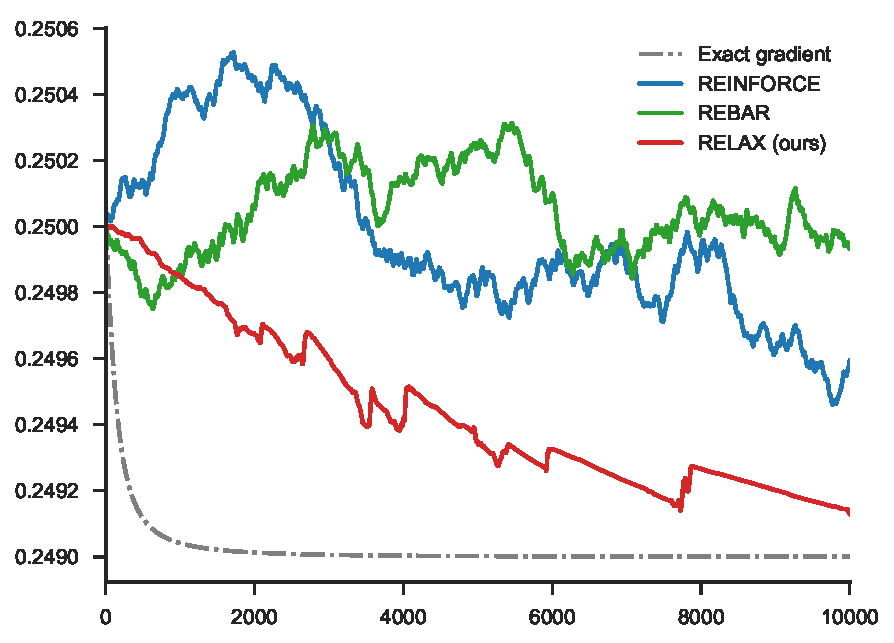
\includegraphics[width=.5\textwidth]{figures/toy_losses_10000_0_499}
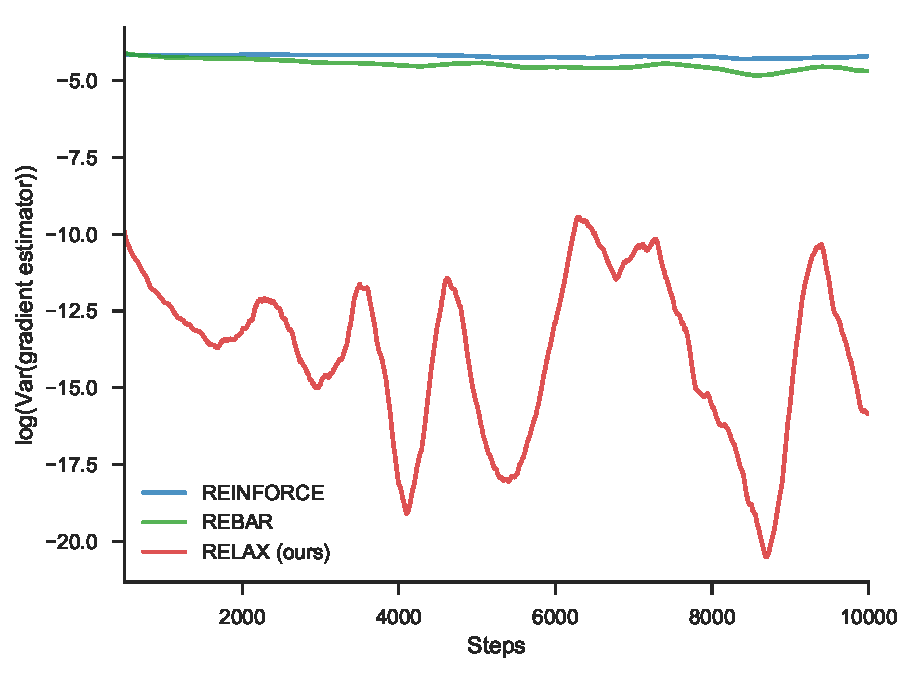
\includegraphics[width=.5\textwidth]{figures/variance_100_t_499}
%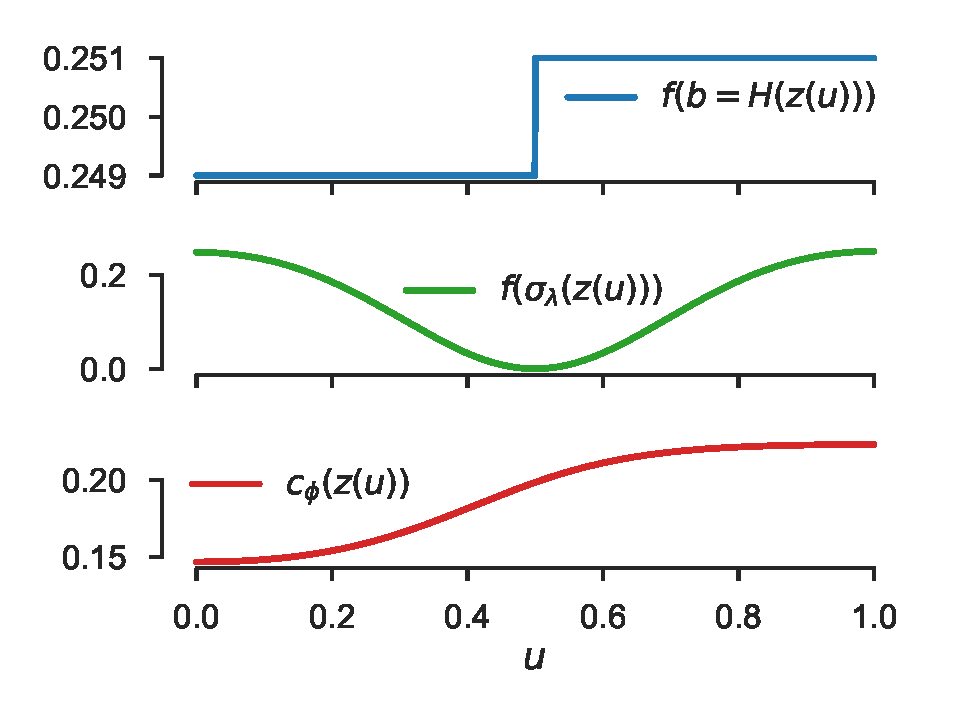
\includegraphics[width=.325\textwidth]{figures/relaxations_t_499_which_2}
\caption{
\emph{Left:} Training curves comparing different gradient estimators on a toy problem: ${\mathcal{L}(\theta) = \E_{p(b|\theta)} [ (b - 0.499)^2 ]}$
\emph{Right:} Variance of each estimator's gradient.
}
\label{first figure}
\end{figure}


\section{Background: Gradient estimators}
How can we choose the parameters of a distribution to maximize an expectation?
This problem comes up in reinforcement learning, where we must choose the parameters $\theta$ of a policy distribution $\pi(a|s, \theta)$ to maximize the expected reward $\mathbb{E}_{\tau \sim \pi} \left[ R \right]$ over state-action trajectories $\tau$.
It also comes up in fitting latent-variable models, when we wish to maximize the marginal probability ${p(x|\theta) = \sum p(x|z) p(z|\theta) = \mathbb{E}_{p(z|\theta)} \left[ p(x|z) \right]}$.
In this paper, we'll consider the general problem of optimizing
%
\begin{align}
\mathcal{L}(\theta)=\expectedLoss{}.
\end{align}
%
%Later, we will discuss the case when $\loss{}$ depends directly on $\theta$.

When the parameters $\theta$ are high-dimensional, gradient-based optimization is a appealing because it provides information about how to adjust each parameter individually.
Stochastic optimization is essential for scalablility, but is only guaranteed to converge to a fixed point of the original objective when the stochastic gradients $\hat g$ are unbiased, i.e. ${\mathbb{E} \left[ \hat g \right] = \PT \mathbb{E}_{p(b|\theta)} \left[ f(b) \right]}$~\citep{robbins1951stochastic}.

%Below we review past work in gradient estimation.
%There are a few general strategies for constructing unbiased gradient estimators:
How can we build unbiased, stochastic estimators of $\PT \mathcal{L}(\theta)$?
There are several standard methods:

\paragraph{The score-function gradient estimator}
One of the most generally-applicable gradient estimators is known as the score-function estimator, or REINFORCE~\citep{williams1992simple}:
%
\begin{align}
\hat g_\textnormal{reinforce} =  f \left( b \right) \PT \log p(b | \theta), \qquad b \sim p(b | \theta)
\end{align}
%
This estimator is unbiased, but in general has high variance.
Intuitively, this estimator is limited by the fact that it doesn't use any information about how $f$ depends on $b$, only on the final outcome $f(b)$.

\paragraph{The reparameterization trick}
When $f$ is continuous and differentiable, and the latent variables $b$ can be written as a deterministic, differentiable function of a random draw from a fixed distribution, the reparameterization trick \citep{williams1992simple, kingma2013autoencoding, rezende2014stochastic} creates a low-variance, unbiased gradient estimator by making the dependence of $b$ on $\theta$ explicit through a reparameterization function $b=T(\theta, \epsilon)$:
%
\begin{align}
%\hat g_\textnormal{reparam} = \frac{\partial f \left( b(\theta, \epsilon) \right)}{\partial \theta}, \qquad \epsilon \sim p(\epsilon)
\hat g_\textnormal{reparam}
= \PT f \left( b \right)
= \frac{\partial f}{\partial T}\frac{\partial T}{\partial \theta} , 
\qquad \epsilon \sim p(\epsilon) 
\end{align}
%
This gradient estimator is often used when training high-dimensional, continuous latent-variable models, such as variational autoencoders or GANs.
One intuition for why this gradient estimator is preferable to REINFORCE is that it depends on $\partial f / \partial b$, which exposes the dependence of $f$ on $b$.
% NOTE for revision: last sentence is confusing. What is the advantage of exposing the dependence of f on b for a gradient estimator?

\paragraph{Control variates}
Control variates are a general method for reducing the variance of a Monte Carlo estimator.
Given an estimator $\hat g(b)$, a control variate is a function $\controlf(b)$ with a known mean $\mathbb{E}_{p(b)} [ \controlf ]$.
Subtracting the control variate from our estimator and adding its mean gives us a new estimator:
%
\begin{align}
\hat g_\textnormal{new}(b) = \hat g(b) - \controlf(b) + \mathbb{E}_{p(b)}[\controlf(b)]
\end{align}
%
This new estimator has the same expectation as the old one:
%
\begin{align}
\mathbb{E}_{p(b)}\left[\hat g_\textnormal{new}(b) \right] 
= \mathbb{E}_{p(b)}\left[\hat g(b) - \controlf(b) + \mathbb{E}_{p(b)} \left[ \controlf(b) \right] \right]
%= \mathbb{E}_{p(b)}\left[f(b) \right] - \mathbb{E}_{p(b)} \left[ \controlf(b) \right] + \mathbb{E}_{p(b)} \left[ \controlf(b) \right]
= \mathbb{E}_{p(b)}\left[ \hat g(b) \right]
\end{align}
%
Importantly, the new estimator has lower variance than $\hat g(b)$ if $\controlf(b)$ is positively correlated with $f(b)$.
% NOTE for revision: 
% I think it's important to stick to the standard definition of a control variate here, which includes the scalar constant eta
% c(b) can be positively or negatively correlated with f(b) and still reduce variance if the control variate has a learned scalar like eta
% Eta can be positive or negative. When you learn eta optimally (Cov(g,c) / Var(c), see for example Tucker et al. 2017 sec. 7.1), eta will flip sign so that even if c(b) is negatively correlated, the new estimator will have lower variance .

\section{Constructing and optimizing a differentiable surrogate}
\label{lax section}
The reparameterization trick, while useful, is only applicable when $f$ is a known, differentiable function of a continuous random variable.
For functions $f$ of discrete variables, gradient estimators based on continuous relaxations such as the concrete, or Gumbel-softmax relaxations~\cite{maddison2016concrete, jang2016categorical} are applicable only when $f$ is known.
%These methods also require that $f$ is known and differentiable with respect to its inputs.
Moreover, they require that $f$ be computable at and behave predictably at inputs outside of the domain of the function.
While these assumptions often hold, they greatly restrict the space of functions for which we can apply these methods. 

In this section, we introduce a gradient estimator for the expectation of a function $\PT \E_{p(b|\theta)}[f(b)]$ that can be applied even when $f$ is unknown, or not differentiable.
%We make no assumptions about the structure of $f$ itself.
This allows the estimator to be applied to a wide range of applications with little or no modification.
Our estimator combines the score function estimator, the reparameterization trick, and control variates.
We obtain an unbiased estimator whose variance can potentially be as low as reparameterization-trick estimator, even when $f$ is not differentiable or not computable.

%We begin with the case where $b$ is a reparameterizable continuous random variable.
%We then handle the case where $b$ is discrete. 

%\subsection{The \LAX{} estimator for continuous random variables}
First, we consider the case where $b$ is continuous, but that $f$ cannot be differentiated.
We begin with the score-function gradient estimator:
%
\begin{align}
\hat g_\textnormal{reinforce} = f \! \left( b \right) \PT \log p(b | \theta), \qquad b \sim p(b|\theta)
\end{align}
%
Instead of differentiating through $f$, we build a surrogate of $f$ using a neural network $c_\phi$, and differentiate $c_\phi$ instead.
Using the fact that the score-function estimator and reparameterization estimator have the same expectation:
%
\begin{align}
\E_{p(\epsilon)} \left[ c_\phi ( b(\epsilon, \theta)) \PT \log p(b | \theta) \right] =
\E_{p(\epsilon)} \left[ \frac{\partial c_\phi}{\partial b} \frac{\partial b(\theta, \epsilon)}{\partial \theta} \right]
\end{align}
%
%
%We first consider the case where $b$ is a continuous random variable.% and then when $b$ is discrete.
%
%\subsection{The \LAX{} estimator -- continuous case} 
%\YW{The symbol $T$ usually refers to sufficient statistics. I don't think we should use it here for reparameterization. Also we should use a lower case letter.}
%We wish to compute $\PT\E_{p(b;\theta)}[f(b)]$ where $p(b;\theta)$ is a distribution with continuous support that admits a reparameterization $b = g_\theta(\epsilon)$, where $\epsilon \sim p(\epsilon)$.
%We assume that $f$ is a black-box, or involves operations such that $\PT f = 0$ almost everywhere or is not computable.
%\YW{This is the motivation for our following proposal. But I find it's not motivated enough.  It sounds like an assumption. But we're actually looking at this type of problem. I suggest motivate this more in the introduction paragraph, background section. List some examples of such $f$.} 
%Given the reparameterization, we can re-write this objective as an expectation over $\epsilon$ as  $\PT\E_{p(\epsilon)}[f(T(\epsilon, \theta)]$.
%
%Let $c_\phi$ be a differentiable function (such as a neural network) parametrized by $\phi$.
%By REINFORCE, we have $\PT\E_{p(b;\theta)}[c_\phi(b)] = \E_{p(b;\theta)}[c_\phi(b)\LP{b;\theta}]$.
%Hence, by adding and subtracting it, we have
%
%\begin{align}
%\PT\E_{p(b;\theta)}[f(b)] &= \E_{p(b;\theta)}\left[ \left[f(b) - c_\phi(b)\right]\cdot\LP{b;\theta}\right]+\PT\E_{p(b;\theta)}[c_\phi(b)]\nonumber\\
%&= \E_{p(\epsilon)} \left[ \left[f(g_\theta(\epsilon)) - c_\phi(g_\theta(\epsilon))\right]\cdot\LP{b} + \PT r(g_\theta(\epsilon))\right]\nonumber
%\end{align}
%
%Which allows us to define our estimator below as: 
%
We can simply add the score-function estimator and subtract the reparameterization estimator, to get:
%
\begin{align}
\label{eq:cont_est}
\hat g_\LAX = \left[ f(b) -c_\phi(b) \right] \PT \log p(b|\theta) + \PT c_\phi(b) \qquad b = T(\theta, \epsilon), \epsilon \sim p(\epsilon).
\end{align}
%
This gives an unbiased estimator for any choice of $c_\phi$.

\subsection{Optimizing the gradient control variate with gradients}

Both presented estimators are unbiased for any choice of the function $c_\phi$, so the only remaining problem is to choose a $c_\phi$ that gives low variance to $\hat g_\LAX$ and $\hat g_\RELAX{}$.
How can we find a $\phi$ which gives our estimator low variance?
We simply optimize $c_\phi$ using stochastic gradient descent, at the same time as we optimize the parameters of our model or policy.

To optimize $c_\phi$, we require the gradient of the variance of our gradient estimator.
To estimate these gradients, we could simply differentiate through the empirical variance over each mini-batch.
Or, following \cite{tucker2017rebar} and \cite{ruiz2016overdispersed}, we can construct an unbiased, single-sample estimator using the fact that our gradient estimator is unbiased.
For any unbiased gradient estimator $\hat g$ with parameters $\phi$:
%
\begin{align}
\PPH \text{Variance}(\hat g)
= \PPH \E[\hat g^2] - \PPH \E[\hat g]^2
%= \PPH \E[\hat g^2] - \PPH \E_{p(b|\theta)}[f(b)]
= \PPH \E[\hat g^2]
= \E \left[ \PPH \hat g^2 \right]
= \E \left[ 2 \hat g \frac{\partial \hat g}{\partial \phi} \right].
\label{eq:vargrad}
\end{align}  % Do we need hats on these gs?  Or get rid of them elsewhere.
%
Thus, an unbiased single-sample estimate of the gradient of the variance of $\hat g$ is given by {$2 \hat g \frac{\partial \hat g}{\partial \phi}$}.

This method of directly minimizing the variance of the gradient estimator stands in contrast to other methods such as Q-Prop~\citep{gu2016q} and advantage actor-critic~\citep{mnih2016asynchronous}, which train the control variate to minimize the squared error $(f(b) - c_\phi(b))^2$.
Our algorithm, which jointly optimizes the parameters $\theta$ and the surrogate $c_\phi$ is given in Algorithm~\ref{lax}.
%[Todo: talk about the variance of the gradient estimator of the variance of the gradient estimators?]

\subsubsection{Optimal surrogate}
What is the form of the variance-minimizing $c_\phi$?
Inspecting the square of \eqref{eq:cont_est}, we can see that this loss encourages $c_\phi(b)$ to approximate $f(b)$, but with a weighting based on $\PT\log p(b)$.  % Todo: reword this awkward sentence.
Moreover, as $c_\phi \rightarrow f$ then $\hat g_\textnormal{\LAX} \rightarrow \PT c_\phi$.
Thus, this objective encourages a balance between the variance of the reparameterization estimator and the variance of the REINFORCE estimator.
Figure~\ref{learned-relaxations} shows the optimal surrogate on a toy problem.


\begin{algorithm}[h]
\begin{algorithmic}
\Require $f(\cdot)$, $\log p(b|\theta)$, reparameterized sampler $b = T(\theta, \epsilon)$, neural network $c_\phi(\cdot)$
\While {not converged} 
	\State $\epsilon_{i} \sim p(\epsilon)$ \Comment Sample noise
	\State $b_i \leftarrow T(\epsilon_i, \theta)$ \Comment Compute input
	\State  $g_\theta \leftarrow \left[f(b_i) - c_{\phi}(b_i) \right] \nabla_\theta \log p + \nabla_\theta c_\phi(b_i)$ \Comment Estimate gradient
	\State  $g_\phi \leftarrow 2 g_\theta \frac{\partial g_\theta}{\partial \phi}$ \Comment Estimate gradient of variance of gradient
	\State $\theta \leftarrow \theta + \alpha_1 g_\theta$ \Comment Update parameters
	\State $\phi \leftarrow \phi + \alpha_2 g_\phi$ \Comment Update control variate
\EndWhile
\State \textbf{return} $\theta$ 
\end{algorithmic}
\caption{\LAX{}: Optimizing parameters and a gradient control variate simultaneously.}
\label{lax}
\end{algorithm}

%\subsection{The \RELAX{} estimator for discrete random variables}
\subsection{Discrete random variables and conditional reparameterization}
We can adapt the \LAX{} estimator to the case where $b$ is a discrete random variable by introducing a ``relaxed'' continuous variable $z$. %, where $b = H(z)$ and $H$ denotes the Heaviside function. %, we 
Here we assume that there exists a continuous, reparameterizable distribution $p(z|\theta)$ and a deterministic mapping $H(z)$ such that $H(z) = b \sim p(b|\theta)$ when $z \sim p(z|\theta)$.
In our implementation, we use the Gumbel-softmax trick, the details of which can be found in appendix~\ref{resample}.

The discrete version of the \LAX{} estimator is given by:
%
\begin{align}
\label{eq:discrete lax}
\hat g_\DLAX = f(b) \PT \log p(b|\theta) - c_\phi(z) \PT \log p(z|\theta) + \PT c_\phi(z), \qquad b = H(z), z \sim p(z|\theta).
\end{align}
%
%When $p(b|\theta)$ is a distribution over discrete random variables, more care must be taken.
This estimator is simple to implement and general.
However, we might expect this estimator to have high variance, since $c_\phi$ must both correlate with the discrete function $f$, whose gradients are zero w.r.t. its input, but also have a low-variance reparameterization gradient.
Intuitively, these two requirements are in direct opposition.

%Most discrete distributions of interest fit into this formulation.
To construct a more powerful gradient estimator, we incorporate a further refinement due to~\cite{tucker2017rebar}.
Specifically, we evaluate our control variate both at a relaxed input $z \sim p(z|\theta)$, and also at a relaxed input \emph{conditioned on the discrete variable $b$}, denoted $\tilde z \sim p(z|b, \theta)$. 
Thus we define our estimator as
%
\begin{align}
\hat g_\textnormal{RELAX} = \left[ f(b) - c_\phi(\hat{z}) \right] \PT \log p(b|\theta) + \PT c_\phi(z) - \PT c_\phi (\tilde{z}) \\
\qquad b = H(z), z \sim p(z|\theta), \tilde{z} \sim p(z|b, \theta) \nonumber
\end{align}
%

\begin{algorithm}[h]
	\begin{algorithmic}
		\Require $f(\cdot)$, $\log p(b|\theta)$, reparameterized samplers $b = T(\theta, \epsilon)$, $z = S(\epsilon, \theta)$ and $\tilde{z} = S(\epsilon, \theta | b)$, \\ 
		\hspace{3em} neural network $c_\phi(\cdot)$  \While {not converged} 
		\State $\epsilon_{i}, \widetilde{\epsilon_i} \sim p(\epsilon)$ \Comment Sample noise
		\State $b_i \leftarrow T(\epsilon_i, \theta)$ \Comment Compute input
		\State $z_i \leftarrow S(\epsilon_i, \theta)$ \Comment Compute unconditional relaxed input
		\State $\widetilde{z_i} \leftarrow S(\widetilde{\epsilon_i}, \theta | b_i)$ \Comment Compute conditional relaxed input
		\State  $g_\theta \leftarrow \left[f(b_i) - c_{\phi}(\widetilde{z_i}) \right] \nabla_\theta \log p + \nabla_\theta c_\phi(z_i) - \nabla_\theta c_\phi(\widetilde{z_i})$ \Comment Estimate gradient
		\State  $g_\phi \leftarrow 2 g_\theta \frac{\partial g_\theta}{\partial \phi}$ \Comment Estimate gradient of variance of gradient
		\State $\theta \leftarrow \theta + \alpha_1 g_\theta$ \Comment Update parameters
		\State $\phi \leftarrow \phi + \alpha_2 g_\phi$ \Comment Update control variate
		\EndWhile
		\State \textbf{return} $\theta$ 
	\end{algorithmic}
	\caption{\RELAX{}: Low-variance control variate optimization for black-box gradient estimation.}
	\label{lax}
\end{algorithm}

This estimator is unbiased for any $c_\phi$.
We prove this following~\cite{tucker2017rebar}:
%
\begin{align}
\E_{p(b|\theta)} \! \left[\left[ f(b) - \E_{p(z|b, \theta)} \! \left[c_\phi(z) \right] \right]\PT \log p(b|\theta)  - \PT \E_{p(z|b, \theta)} \! \left[c_\phi(z) \right] \right] + \PT\E_{p(z|\theta)} \! \left[ c_\phi(z) \right] \span & \nonumber\\
&= \PT \E_{p(b|\theta)} \! \left[ f(b) - \E_{p(z|b, \theta)}\left[ c_\phi(z) \right]  \right] + \PT\E_{p(z|\theta)} \! \left[ c_\phi(z) \right]\nonumber\\
&= \PT \E_{p(b|\theta)} \! \left[ f(b) \right] - \PT\E_{p(z|\theta)} \! \left[ c_\phi(z) \right] + \PT\E_{p(z|\theta)} \! \left[ c_\phi(z) \right]
= \PT \expectedLoss{}%&= \E_{p(\epsilon, \hat{\epsilon})}\Big[\left( f(H(T(\epsilon, \theta))) - c_\phi(T(\epsilon, \theta))  \right) \PT \log p(H(T(\epsilon, \theta))|\theta) - \PT c_\phi(\hat{T}(\hat{\epsilon}, H(T(\epsilon, \theta)), \theta)) \Big]\nonumber\\
%&\qquad + \PT\E_{p(\epsilon)}\left[ c_\phi(T(\epsilon, \theta)) \right]
\end{align}
%
We note that the distribution $p(z|b,\theta)$ must also be reparameterizable.
This is the case for Bernoulli and categorical random variables.
We demonstrate how to perform this conditional reparameterization in appendix~\ref{resample}.

\subsection{Choosing the control variate architecture}
%We have introduced a generic family of algorithms which produce unbiased and potentially low variance estimates of $\PT \E_{p(b|\theta)}[f(b)]$.
%Furthermore, we provide a tractable method to optimize the parameters of the control variate to minimize the variance of the estimator.
%Our approach allows us to design our control variate $c_\phi$ in any way we please.
The variance-reduction objective introduced above allows us to use any differentiable, parametric function as our control variate $c_\phi$. 
How should we choose the architecture of $c_\phi$?
Ideally, we will take advantage of any known structure in $f$.

If $f$ is a known, differentiable function of discrete random variables, we can use the concrete relaxation~\cite{maddison2016concrete} and let $c_\phi(z) = f(\sigma_\lambda(z))$.
In this special case, our estimator is exactly the REBAR estimator.
We are also free to add a learned component to the concrete relaxation and let $c_\phi(z) = f(\sigma_\lambda(z)) + \hat{r}_\rho(z)$ where $\hat{r}_\rho$ is a neural network with parameters $\rho$.
We have taken this approach in our experiments training discrete variational auto-encoders.
If no information about $f$ is known, then we are also free to let $c_\phi$ be a generic function approximator such as a neural network.
This is the approach we have taken in our reinforcement learning experiments.


%\section{Conditional reparameterization}
%\label{conditional reparam section}
%To apply our method to discrete random variables, we incorporate a further refinement, based on a technique adapted from the REBAR method of \citet{tucker2017rebar}.
%First, we must introduce another 
%%
%
%A similar relaxation for the Bernoulli distribution has been developed as well (see Appendix for details)
%This gradient estimator is fairly effective in practice, but produces biased gradients, hindering its usage.
%Additionally, it is not clear how to set the temperature $\lambda$ and it is often treated as a hyperparameter.
%
%\paragraph{REBAR}
%REBAR gives unbiased estimates of the gradient of expectations of known functions of Bernoulli random variables.
%This method uses the REINFORCE estimator with a control variate.
%The control variate is derived from the original loss function evaluated at continuously-relaxed inputs \citep{maddison2016concrete, jang2016categorical}.
%The expectation of this control variate is estimated with low variance via the reparameterization trick. 
%
%\paragraph{Concrete relaxation}
%When $b$ is discrete and $f$ is known, one general approach is to differentiate a continuous relaxation of the discrete random variables.
%\cite{maddison2016concrete} and \cite{jang2016categorical} developed a differentiable relaxation of the categorical distribution, called the concrete distribution:
%
%\begin{align}
%\hat g_\textnormal{concrete} = \PT f \left( \sigma_\lambda ( \log \theta - \log(-\log u)) \right), \qquad u \sim \textnormal{uniform}[0, 1] 
%\end{align}
%
%where $\sigma_\lambda$ is the \texttt{softmax} function with temperature $\lambda$.
%
%Samples are drawn from $p(b|\theta)$ with a deterministic function of a continuous, reparameterizable random variable $z$. 
%
%\begin{align}
%z &:= g(u, \theta) = \log\frac{\theta}{1-\theta} + \log\frac{u}{1-u}, \qquad u \sim \text{uniform}[0,1]\nonumber\\
%b &:= \mathbb{I}(z>0)\nonumber
%\end{align}
%
%Thus, we can think of $p(b|\theta)$ as $\int p(b|z, \theta)p(z|\theta)dz$. The REBAR estimator is derived from this realization, noting:
%\begin{align}
%\PT \expectedLoss{} &= \PT \E_{p(b|\theta)}\left[ f(b) \right] - \PT\E_{p(z|\theta)}\left[ f(\sigma_\lambda(z) \right] + \PT\E_{p(z|\theta)}\left[ f(\sigma_\lambda(z) \right]\nonumber\\
%&= \PT \E_{p(b|\theta)}\left[ f(b) - \PT\E_{p(z|b, \theta)}\left[ f(\sigma_\lambda(z) \right]  \right] + \PT\E_{p(z|\theta)}\left[ f(\sigma_\lambda(z) \right]\nonumber\\
%&= \E_{p(b|\theta)}\left[\left( f(b) - \E_{p(z|b, \theta)}\left[ f(\sigma_\lambda(z) \right] \right)\PT \log p(b|\theta)  - \PT \E_{p(z|b, \theta)}\left[ f(\sigma_\lambda(z) \right] \right]\nonumber\\
%&\qquad + \PT\E_{p(z|\theta)}\left[ f(\sigma_\lambda(z) \right]\nonumber
%\end{align}
%
%where $\sigma_\lambda$ is the sigmoid function with temperature $\lambda$.
%The REBAR estimator is the single-sample monte-carlo estimator derived from the last line above.
%The REBAR estimator is computed as:
%\begin{align}
%\hat g_\textnormal{REBAR} = \left(f(b) - f(\sigma_\lambda(z)\right)\PT \log p(b|\theta) + \PT f(\sigma_\lambda(z)) - \PT f(\sigma_\lambda(\tilde{z}))\nonumber\\
%z \sim p(z|\theta), \tilde{z} \sim p(z|b, \theta), b = \mathbb{I}(z>0)\nonumber
%\end{align}
%Details of how to sample from $p(z|b, \theta)$ as well as an extension to categorical random variables can be found in the Appendix.
%\cite{tucker2017rebar} also introduced a way to optimize the temperature parameter $\lambda$ via gradient decent to minimize the variance of the estimator. 



%In the case where $p(b|\theta)$ is a distribution over discrete variables, a few more details arise.
%In this section, we first review the technique of concrete relaxation introduced in \cite{maddison2016concrete} and \cite{jang2016categorical}. 
%Inspired by REBAR \citet{tucker2017rebar}, we propose a more general family of gradient estimators called \RELAX{} for discrete variables. 

%We mainly consider the most commonly used discrete distribution, the Categorical distribution (which includes Bernoulli distribution as a special case).
%A well-known approach to obtain a sample from a Categorical distribution with probability vector $\theta = \{\theta_i\}_1^k$ is by
%\begin{align}
%z &= \log\theta - \log(-\log u),\qquad u \sim \text{uniform}[0,1]^k\nonumber \\
%b &= H(z), \nonumber
%\end{align}
%where $H(\cdot)$ is the \texttt{argmax} function. Inspired by REBAR \citet{tucker2017rebar}, we write $p(z|\theta)$ as $\int p(z|b, \theta)p(b|\theta)db$. Note that if $p(z|\theta)$ and $p(z|b, \theta)$ are reparameterizable, i.e., there exists $\hat{T}$ such that $\hat{T}(\hat{\epsilon}, b, \theta) = \hat{z} \sim p(z|b, \theta)$. See Appendix for details on sampling from $p(z|b, \theta)$ in both the Bernoulli and Categorical cases.
%As in \LAX{}, we let $c_\phi$ be an differentiable function. Now we derive our estimator as follows,
%
%\begin{align}
%\PT \expectedLoss{} &= \PT \E_{p(b|\theta)}\left[ f(b) \right] - \E_{p(z|\theta)}\left[ c_\phi(z) \right] + \PT\E_{p(z|\theta)}\left[ c_\phi(z) \right]\nonumber\\
%&= \PT \E_{p(b|\theta)}\left[ f(b) - \E_{p(z|b, \theta)}\left[ c_\phi(z) \right]  \right] + \PT\E_{p(z|\theta)}\left[ c_\phi(z) \right]\nonumber\\
%&= \E_{p(b|\theta)}\left[\left( f(b) - \E_{p(z|b, \theta)}\left[c_\phi(z) \right] \right)\PT \log p(b|\theta)  - \PT \E_{p(z|b, \theta)}\left[c_\phi(z) \right] \right]\nonumber\\
%&\qquad + \PT\E_{p(z|\theta)}\left[ c_\phi(z) \right]\nonumber\\
%&= \E_{p(\epsilon, \hat{\epsilon})}\Big[\left( f(H(T(\epsilon, \theta))) - c_\phi(T(\epsilon, \theta))  \right) \PT \log p(H(T(\epsilon, \theta))|\theta) \nonumber\\
%&\qquad\qquad\qquad - \PT c_\phi(\hat{T}(\hat{\epsilon}, H(T(\epsilon, \theta)), \theta)) \Big]\nonumber\\
%&\qquad + \PT\E_{p(\epsilon)}\left[ c_\phi(T(\epsilon, \theta)) \right]\nonumber
%\end{align}
%
%which allows us to define our estimator as
%
%\begin{align}
%\hat g_\textnormal{RELAX} = \left(f(b) -c_\phi(\hat{z})\right)\PT \log p(b|\theta) + \PT c_\phi(z) - \PT c_\phi (\tilde{z}) \nonumber\\
%\qquad b = H(z), z \sim p(z|\theta), \tilde{z} \sim p(z|b, \theta)
%\end{align}
%
%This estimator is also unbiased i.e $E_{\epsilon, \hat{\epsilon}}[g_\phi] = \PT\E_{p(b|\theta)}[f(b)]$.
%Therefore we can take the advantage of reparameterization to further reduce the variance of the estimator.


\subsection{Reinforcement learning}
We now describe how we apply the \LAX{} estimator in the reinforcement learning (RL) setting.
By reinforcement learning, we refer to the problem of optimizing the parameters $\theta$ of a policy distribution $\pi(a | s, \theta)$ to maximize the sum of rewards.
In this setting, the random variable being integrated over is $\tau$, which denotes a series of actions and states $[(s_1, a_1), (s_2, a_2), ..., (s_T, a_T)]$.
The function whose expectation is being optimized, $R$, maps $\tau$ to the sum of rewards ${R(\tau) = \sum_{t=1}^{T} r_t(s_t, a_t)}$.

Again, we want to estimate the gradient of an expectation of a black-box function: $\nicefrac{\partial \mathbb{E}_{p(\tau|\theta)}[R(\tau)]}{\partial \theta}$.
The \emph{de facto} standard approach is the advantage actor-critic estimator (A2C)~\citep{sutton2000policy}:% which is the standard policy gradient algorithm. 
%We seek to compute
%
%\begin{align}
%\frac{\partial \E_\tau[R]}{\partial \theta} = \E \left[ \sum_{t=1}^{\infty} \LL{t} \sum_{t'=t}^{\infty} r_t \right]
%\end{align}
%
%but the estimator on the right hand side can have potentially high variance.
%
%We can view the sum of future rewards as a black-box function of state-action trajectories $\tau$ sampled from our policy.
%Instead, we typically compute
%
%\begin{align}
%\frac{\partial \E_\tau[R]}{\partial \theta} = \E_\tau \left[ \sum_{t=1}^{\infty} \LL{t} \left[ \sum_{t'=t}^{\infty} r_{t'} - b(s_t) \right] \right]
%\end{align}
%
%
\begin{align}
\hat g_{\textnormal{A2C}} = \sum_{t=1}^{\infty} \LL{t} \left[ \sum_{t'=t}^{\infty} r_{t'} - c_\phi(s_t) \right]+\frac{\partial}{\partial\theta} c_\phi(s_t), \qquad a_t \sim \pi(a_t | s_t, \theta)
\label{eq:rl_a2c}
\end{align}
%
Where $c_\phi(s_t)$ is an estimate of the state-value function, $c_\phi(s) \approx V^\pi(s) = \E_{\tau}[R|s_1=s].$
This estimator is unbiased when $c$ does not depend on $a_t$.
The main limitations of A2C are that $c$ does not depend on $a_t$, and that it's not obvious how to optimize $c$.
Using the \LAX{} estimator addresses both of these problems.

First, we assume $\pi(a_t|s_t)$ is reparametrizable, meaning that we can write $a_t = a(\epsilon_t, s_t, \theta)$, where $\epsilon_t$ does not depend on $\theta$.
We again introduce a differentiable surrogate $c_\phi(a,s)$.
Crucially, this surrogate is a function of the action as well as the state.

Our estimator is defined as: 
%
\begin{align}
\hat g_\LAX^{\RL} = \sum_{t=1}^{\infty} \LL{t} \left[ \sum_{t'=t}^{\infty} r_{t'} - c_\phi(a_t,s_t) \right] +\frac{\partial}{\partial\theta} c_\phi(a_t, s_t), \\
a_t = a(\epsilon_t,s_t, \theta) \qquad \epsilon_t \sim p(\epsilon_t)\nonumber.
\label{eq:rl_est}
\end{align}
%
This estimator is unbiased if the true dynamics of the system are Markovian w.r.t. the state $s_t$.
When $T = 1$, we recover the special case ${\hat g_\LAX^{\RL} = \hat g_\LAX}$.
Comparing $\hat g_\LAX^{\RL}$ to the standard advantage actor-critic estimator in~\eqref{eq:rl_a2c}, the main difference is that our baseline $c_\phi(a_t, s_t)$ is action-dependent while still remaining unbiased.

To optimize the parameters $\phi$ of our control variate $c_\phi(a_t, s_t)$, we can again use the single-sample estimator of the gradient of our estimator's variance given in~\eqref{eq:vargrad}.
This approach avoids unstable training dynamics, and doesn't require storage and replay of previous rollouts.

Details of this derivation, as well as the discrete and conditionally reparameterized version of this estimator can be found in appendix~\ref{rl appendix}.

\section{Scope and Limitations}
\label{limitations}
%\YW{For this section we can focus on comparisons to REBAR, because it is the most related one which might also raise most questions. We can briefly mention previous methods for doing discrete variables. We should also mention Q-prop.}
The recently-developed REBAR method~\citep{tucker2017rebar} is the work most related to ours.
REBAR estimates the gradient of expectations of functions of Bernoulli random variables.
This method uses the REINFORCE estimator with a control variate.
The control variate is derived from the original loss function evaluated at continuously-relaxed inputs~\citep{maddison2016concrete, jang2016categorical}.
The expectation of this control variate is estimated with low variance via the reparameterization trick.
The REBAR estimator can been seen as a special case of the RELAX estimator when ${c_\phi(z) = f(\sigma_\lambda(z))}$.
%While the above approaches have greatly broadened the scope of functions whose derivatives we can approximate, there still exist a number of factors limiting their application to many problems of interest.

%The bias induced by the concrete relaxation can lead to convergence at unsuitable optima or no convergence at all.
%REBAR alleviates these issues by using the relaxation as a control variate for the estimator instead of using it as the estimator itself.
Unfortunately, REBAR and concrete require the function being optimized, whose input is only defined at discrete inputs, to also accept continuous inputs, be differentiable w.r.t. those inputs, and behave predictably with respect to those continuous inputs.
While often true, these are strong assumptions to make.
Furthermore, REBAR and concrete require that the function being optimized is known. 
This makes REBAR and the concrete relaxation inapplicable for optimizing black-box functions, as in reinforcement learning settings where the reward is an unknown function of the environment.

In contrast, \LAX{} and \RELAX{} can be used in these settings.
\LAX{} and \RELAX{} only require that we can query the function being optimized, and can sample from and differentiate $p(b|\theta)$.

Can \RELAX{} be used to optimize deterministic black-box functions?
The answer is yes, with the caveat that one must introduce stochasticity to the inputs.
Thus, \RELAX{} is most suitable for problems where one is already optimizing a distribution over inputs, such as in inference or reinforcement learning.
% Note that most optimal policies are deterministic?

In our previous analysis, we have made the assumption that the function $f$ we are optimizing is not a function of $\theta$. Oftentimes a dependence on $\theta$ can arise naturally (as in the ELBO) or as a regularizer (such as weight-decay). If $f$ does depend on $\theta$ we note:
\begin{align}
\PT \E_{p(b|\theta)}[f(b, \theta)] = \E_{p(b|\theta)}\left[\PT f(b, \theta) + f(b, \theta)\PT \log p(b|\theta) \right].\nonumber
\end{align}
The second term on the right-hand side can be estimated using any of the methods presented in this paper and if $f$ is known and differentiable then the left-hand side can be computed by back-propagation.


\section{Related work}
There has been a great deal of other recent work in the area of gradient estimation.
\citet{miller2017reducing} reduce the variance of reparameterization gradients in an orthogonal way to ours by approximating the gradient-generating procedure with a simple model and using that model as a control variate.
NVIL~\citep{mnih2014neural} and VIMCO~\citep{mnih2016variational} provide reduced variance gradient estimation in the special case of discrete latent variable models and discrete latent variable models with Monte-Carlo objectives.
\citet{salimans2017evolution} estimate gradients using a form of finite differences, evaluating hundreds of different parameter values in pararallel to construct a gradient estimator.
In contrast, our method is a single-sample estimator.

%As gradient estimators become more complex, checking their unbiasedness numerically becomes difficult.
%The automatic theorem-proving-based unbiasedness checker developed by \citet{selsam2017developing} may become relevant to this line of research.

%Also: \citep{levine2016end}

\citet{staines2012variational} address the general problem of developing gradient estimators for deterministic black-box functions or discrete optimization.
They introduce a sampling distribution, and optimize an objective similar to ours.
\citet{wierstra2014natural} also introduce a sampling distribution to build a gradient estimator, and consider optimizing the sampling distribution.

In the reinforcement learning setting, the work most similar to ours is $Q$-prop \cite{haarnoja2017reinforcement}.
Like our method, $Q$-prop reduces the variance of the policy gradient with an learned, action-dependent control variate whose expectation is approximated via a monte-carlo sample from a taylor series expansion of the control variate.
Unlike our method, their control variate is trained off-policy. While our method is applicable in both the continuous and discrete action domain, $Q$-prop is only applicable in environments with continuous actions. We are interested in the potential of training our control variate off-policy, but we leave that for further work. 

%\citet{asadi2017mean} reduce the variance of actor-critic gradient estimates by simply summing over all possible actions.

%\par{Generalized Reparameterization Gradients}
%REBAR and the generalization in this paper uses a mixture of score function and reparameterization gradients.
%A recent paper by \cite{ruiz2016generalized} unifies these two gradient estimators as the generalized reparameterization gradient (GRG).
%This framework can help disentangle the various components of generalized REBAR.

%REBAR innovation as further decomposition the correction term into secondary reparameterization components
%note this is a recursive application of the principles of GRG
%observe that the GRG suggests this recursive application to components of an estimator
%propose that other estimators could be similarly recursively decomposed?


\section{Applications}
\label{Applications}
We demonstrate the effectiveness of our estimator on a number of challenging optimization problems. Following~\citet{tucker2017rebar} we begin with a simple toy example to illuminate the potential of our method and then continue to the more relevant problems of optimizing binary VAE's and reinforcement learning.

\subsection{Toy experiment}
\begin{wrapfigure}[]{R}{0.50\textwidth}
	\centering
		\vspace{-3mm}
	\hspace{-2.5mm}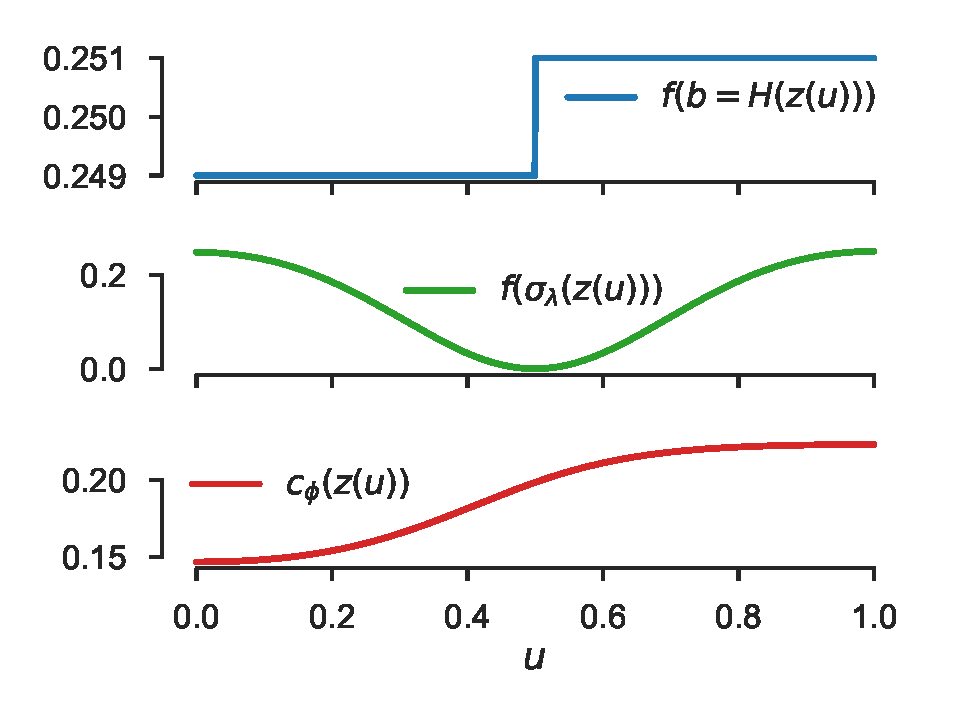
\includegraphics[width=0.50\columnwidth ]{figures/relaxations_t_499_which_2} 
		\vspace*{-6mm}
	\caption{ The relaxation for a toy loss function ${\mathcal{L}(\theta) = \E_{p(b|\theta)} [ (b - 0.499)^2 ]}$ using REINFORCE (blue), REBAR (green), and RELAX (red)} 
	\label{learned-relaxations}
\end{wrapfigure}
We seek to minimize $\mathbb{E}_{p(b|\theta)}[(b - t)^2]$ as a function of the parameter $\theta$ where {$p(b|\theta) = \textnormal{Bernoulli}(b|\theta)$}. \cite{tucker2017rebar} set the target $t = .45$.
We focus on the more challenging case where $t = .499$.
Figures~\ref{first figure}a and \ref{first figure}b and shows the relative performance and gradient variance of REINFORCE, REBAR, and RELAX.

%With this setting of the target, REBAR and competing methods suffer from high variance and are unable to discover the optimal solution $\theta = 0$.
%The fixed concrete relaxation of REBAR is unable to produce a gradient whose signal outweighs the sample noise and is therefore unable to solve this problem noticeably faster than REINFORCE.

Figure~\ref{learned-relaxations} plots the learned surrogate $c_\phi$ for a fixed value of $\theta$. We can see that $c_\phi$ is near $f$ for all $z$, keeping the variance of the REINFORCE part of the estimator small. Moreover the derivative of $c_\phi$ is positive for all $z$ meaning that the reparameterization part of the estimator will produce gradients pointing in the correct direction to optimize the expectation. Conversely, the concrete relaxation of REBAR is close to $f$ only near $0$ and $1$ and its gradient points in the correct direction only for values of $z > t$. These factors together result in the RELAX estimator achieving the best performance. 

\subsection{Discrete variational autoencoder}
Next, we evaluate the \RELAX{} estimator on the task of training a variational autoencoder~\citep{kingma2013autoencoding, rezende2014stochastic} with Bernoulli latent variables.
We reproduced a subset of the experiments from \citet{tucker2017rebar}, training models with 1 and 2 layers of 200 Bernoulli random variables with linear mappings between them, on both  the MNIST and Omniglot~\citep{lake2015human} datasets.
Details of these models and our experimental procedure can be found in appendix~\ref{app_disc_vae}.

%them and a model with 1 layer of Bernoulli random variables with non-linear mappings between layers.

To take advantage of the available structure in the loss function, we choose the form of our control variate to be $$ c_\phi(z) = f(\sigma_\lambda(z))+  \hat{r}_\rho(z) $$ where $\hat{r}_\rho$ is a neural network with parameters $\rho$ and $f(\sigma_\lambda(z))$ is the discrete loss function (the evidence lower-bound) evaluated at continuously relaxed inputs as in REBAR.  
%We found that due to the complicated structure of the loss function, the RELAX estimator performed worse than REBAR. Instead we add a learned relaxation to REBAR's control variate which we denote relaxed-REBAR.
%Our estimator takes the form of \eqref{eq:RELAX} with $$\bar \relaxed(z) = \relaxed(z) + f(\sigma_\lambda(z))$$ where $\relaxed(z)$ is a learned neural network and $f(\sigma_\lambda(z))$ is the Concrete relaxation of REBAR with temperature parameter $\lambda$.
%
%We compare  \cite{tucker2017rebar}.
In all experiments, the learned control variate improved the training and validation performance, over the state-of-the-art baseline of REBAR. 

\begin{table}[h]
\centering
\begin{tabular}{r l | c c c c c} 
Dataset & Model & Concrete & NVIL & MuProp  & REBAR & RELAX\\\midrule
%Nonlinear      & $-102.2$ & $-101.5$ & -101.1  &  -81.01 &  \textbf{-78.13} \\
\textbf{MNIST} & 1 layer  &-111.3 & $-112.5$ & $-111.7$  & -111.6 & \textbf{-111.20} \\ 
               & 2 Layer  &-99.62 & $-99.6$ & $-99.07$   & -98.22 & \textbf{-98.00} \\
\midrule
%Nonlinear      & $-110.4$  & $-109.58$ & -108.72  & -62.28 & \textbf{-58.55} \\
\textbf{Omniglot} & 1 layer &-117.23 & $-117.44$ & $-117.09$   & -116.63 & \textbf{-116.57} \\ 
                  & 2 Layer &-109.95 & $-109.98$ & $-109.55$  & -108.71 & \textbf{-108.54}
\end{tabular}
\caption{Best obtained training objective.}
\label{tab:vae tr}
\end{table}


\begin{table}[h]
\centering
\begin{tabular}{r l | c c} 
  Dataset & Model & REBAR & RELAX \\\midrule
\textbf{MNIST} & 1 layer  & -114.32 & \textbf{-113.62} \\ 
& 2 Layer  & -101.20 & \textbf{-100.85} \\ \midrule
\textbf{Omniglot} & 1 layer & -122.44 & \textbf{-122.11} \\ 
& 2 Layer & -115.83 & \textbf{-115.42}
\end{tabular}
\caption{Best obtained validation objective.}
\label{tab:vae val}
\end{table}

%In \citep{tucker2017rebar}, a separate REBAR estimator was used to estimate the gradients of each model parameter (each weight matrix and bias vector).
%To apply our estimator to this formulation, we would need to learn a separate relaxation for each model parameter.
%To get around this, we use our gradient estimator to approximate $g_\phi \approx \PT \E_{q(b|\theta)}[f(b)]$ where $x\cdot W = \theta$ is the parameters of the Bernoulli latent variables, $W$ is our layer's weight matrix. We then obtain an estimate of $\PP{W} \E_{q(b|\theta)}[f(b)] = g_\phi\cdot \frac{\partial \theta}{\partial W}$. We note this gives us unbiased gradients because 
%\begin{align}
%\E_\epsilon[g_\phi(\epsilon) \cdot \frac{\partial \theta}{\partial W}] = \E_\epsilon[g_\phi(\epsilon)] \cdot \frac{\partial \theta}{\partial W} =  \PT \E_{q(b|\theta)}[f(b)] \cdot \frac{\partial \theta}{\partial W} = 
%\frac{\partial}{\partial W} \E_{q(b|\theta)}[f(b)]
%\end{align} 

%To provide a fair comparison, we re-implemented REBAR in this way (denoted REBAR-ours in table~\ref{tab:vae}).
%We believe this explains the large difference in performance between our implementation and that of \citep{tucker2017rebar} for the nonlinear models since there are 3 layers of parameters that all share the same gradient estimator.
%In the linear models, each layer has its own gradient estimator making our implementation closer to that of \citep{tucker2017rebar}.
To obtain training curves we created our own implementation of REBAR, which gave identical or slightly improved performance to compared the implementation of \citet{tucker2017rebar}.

While we obtained a modest improvement in training and validation scores (tables~\ref{tab:vae tr} and \ref{tab:vae val}), the most notable improvement provided by \RELAX{} is in its rate of convergence.
Training curves for all models can be seen in figures~\ref{fig:vae mnist} and \ref{fig:vae omni}.
In table~\ref{tab:vae epochs} we compare the number of training epochs that are required to match the best validation score of REBAR.
In all experiments, RELAX provides an increase in rate of convergence. 

\begin{figure}[h]
\centering
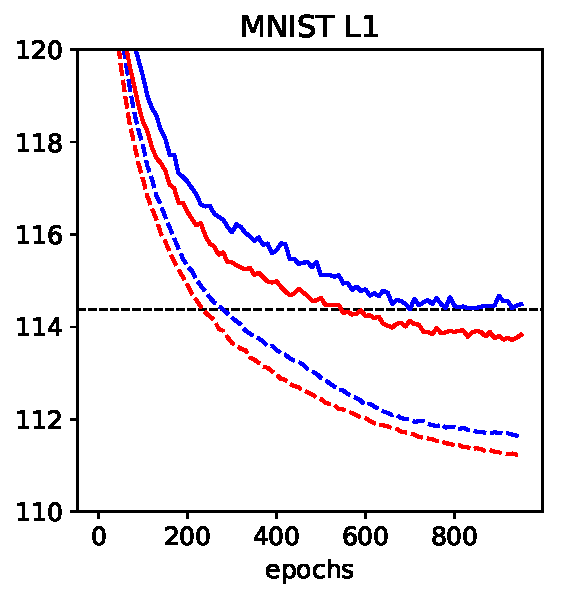
\includegraphics[width=.4\textwidth]{figures/MNIST_L1}
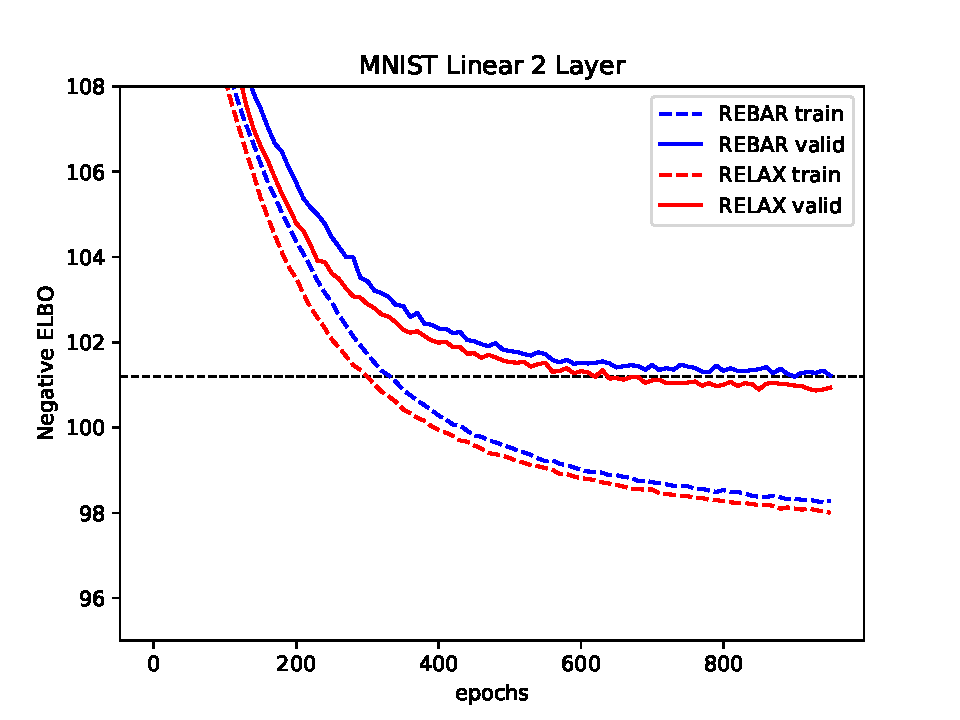
\includegraphics[width=.4\textwidth]{figures/MNIST_L2}
\caption{Training curves on MNIST. The horizontal dashed line indicates the lowest validation error obtained by REBAR.}
\label{fig:vae mnist}
\end{figure}

\begin{figure}[h]
\centering
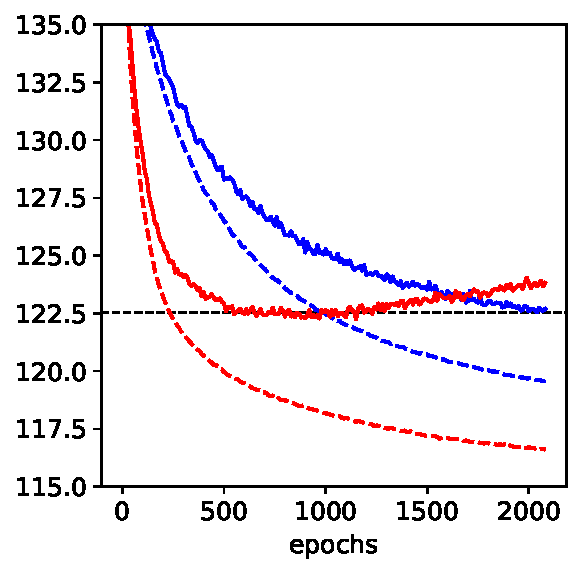
\includegraphics[width=.4\textwidth]{figures/OMNIGLOT_L1}
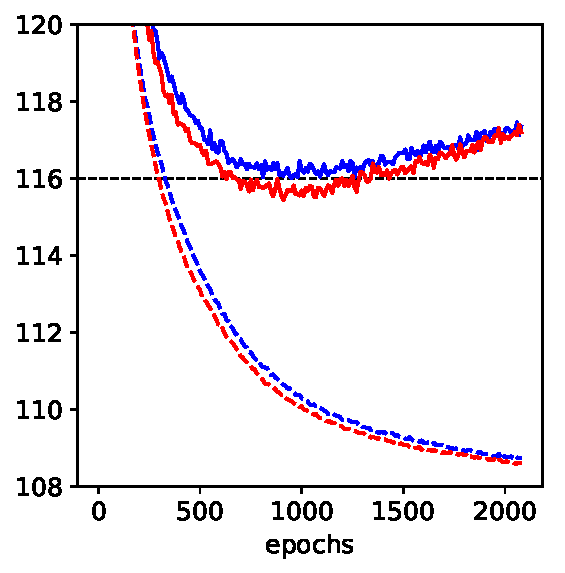
\includegraphics[width=.4\textwidth]{figures/OMNIGLOT_L2}
\caption{Training curves on OMNIGLOT. The horizontal dashed line indicates the lowest validation score obtained by REBAR.}
\label{fig:vae omni}
\end{figure}

\begin{table}[h]
\centering
\begin{tabular}{r l | c c} 
 Dataset & Model  & REBAR & RELAX \\\midrule
\textbf{MNIST} & 1 layer  & 857 & \textbf{531} \\ 
& 2 Layer  & 900 & \textbf{620} \\
\midrule
\textbf{Omniglot} & 1 layer & 2086 & \textbf{566} \\ 
& 2 Layer & 1027 & \textbf{673}
\end{tabular}
\caption{Epochs needed to achieve REBAR's best validation score.}
\label{tab:vae epochs}
\end{table}



\subsection{Reinforcement learning}
We apply our gradient estimator to a few simple reinforcement learning environments with discrete and continuous actions.
We use the \RELAX{} and \LAX{} estimators for discrete and continuous actions, respectively.
We compare with the advantage actor-critic algorithm (A2C)~\cite{sutton2000policy} as a baseline. Full details of our experiments can be found in Appendix~\ref{experiment appendix}.

% <Dami: i took it out because it doesn't match with the continuous case, and we dont' have variance plots yet>We are aware that better results could be obtained with bootstrapping and larger batch sizes but we wanted to work in the highest possible variance setting to demonstrate the variance reduction capabilities of our approach.

%We test our alrgorithm on the Cart-Pole and Lunar-Lander environments from the OpenAI Gym~\cite{1606.01540}.
%We run the Cart-Pole and Lunar-Lander environments for 250 and 1000 episodes, respectively and plot reward and the log-variance of the policy gradients in figure~X.

\subsubsection{Experiments}

In the discrete action setting, we test our approach on the Cart Pole and Lunar Lander environments as provided by the OpenAI gym~\cite{1606.01540}. In the continuous action setting, we test on the MuJoCo~\cite{todorov2012mujoco}-simulated environments Inverted Pendulum and Inverted Double Pendulum also found in the OpenAI gym.

In all tested environments we observe improved performance and sample efficiency using our method. The results of our experiments can be seen in figures \ref{fig:disc_rl}, [CITE OTHER RELEVANT FIGURES] and table~\ref{tab:rl_results}.

We found that our estimator produced policy gradients with drastically reduced variance (see figure~\ref{fig:disc_rl_var}) allowing for larger learning rates to be used while maintaining stable training. In both discrete environments our estimator achieved an over 2-times speedup in convergence over the baseline.



\begin{table}[h]
\centering
\begin{tabular}{l | c c c c } 
\textbf{Model} & Cart Pole & Lunar Lander & Inverted Pendulum & Inverted Double Pendulum \\\midrule
A2C             & $1152 \pm 90$ & $162374 \pm 17241$                    & $9916 \pm 235$ & $78260 \pm 1877$  \\
LAX/RELAX & $\bm{472 \pm 114}$ & $\bm{68712 \pm 20668}$ & $\bm{6237 \pm 45}$ & $\bm{60967 \pm 1669}$\\\\
\end{tabular}
\caption{Mean Episodes to Solve. Cart Pole is solved if the agent receives an average reward over $195$ in the last $100$ Episodes. Lunar Lander is solved if the agent receives an average reward over $200$ in the last $100$ frames. Inverted Pendulum is solved if the agent receives an average reward over $950$ in the last $100$ Episodes. Inverted Double Pendulum is solved if the agent receives an average reward over $9100$ in the last $100$ frames.}
\label{tab:rl_results}
\end{table}

\begin{figure}[h]
\centering
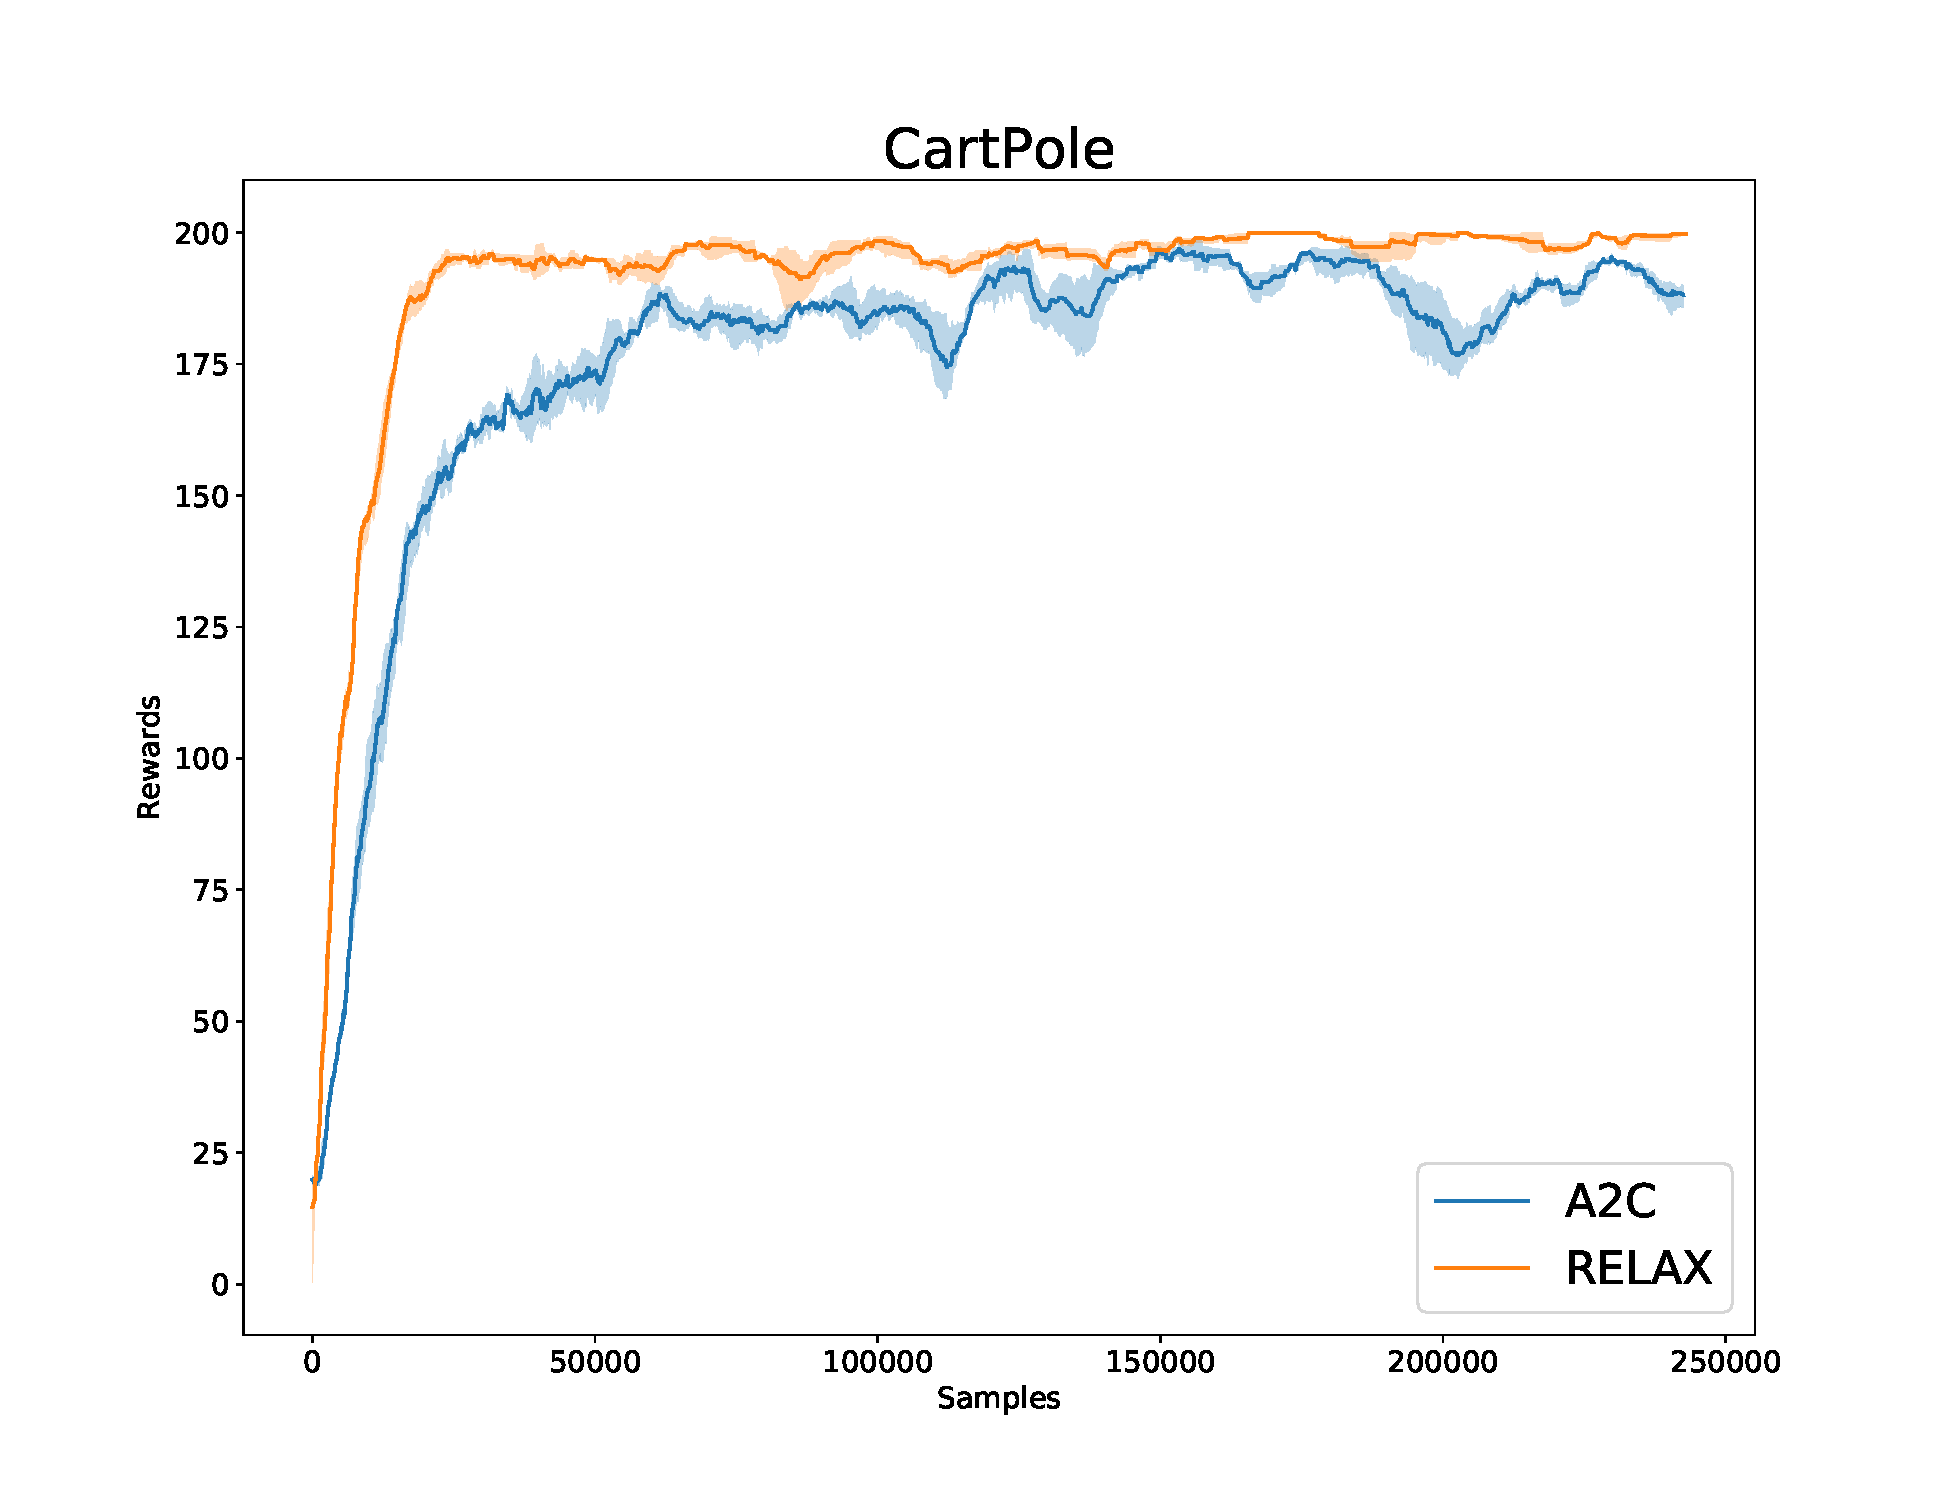
\includegraphics[width=.22\textwidth]{figures/cp_paper}
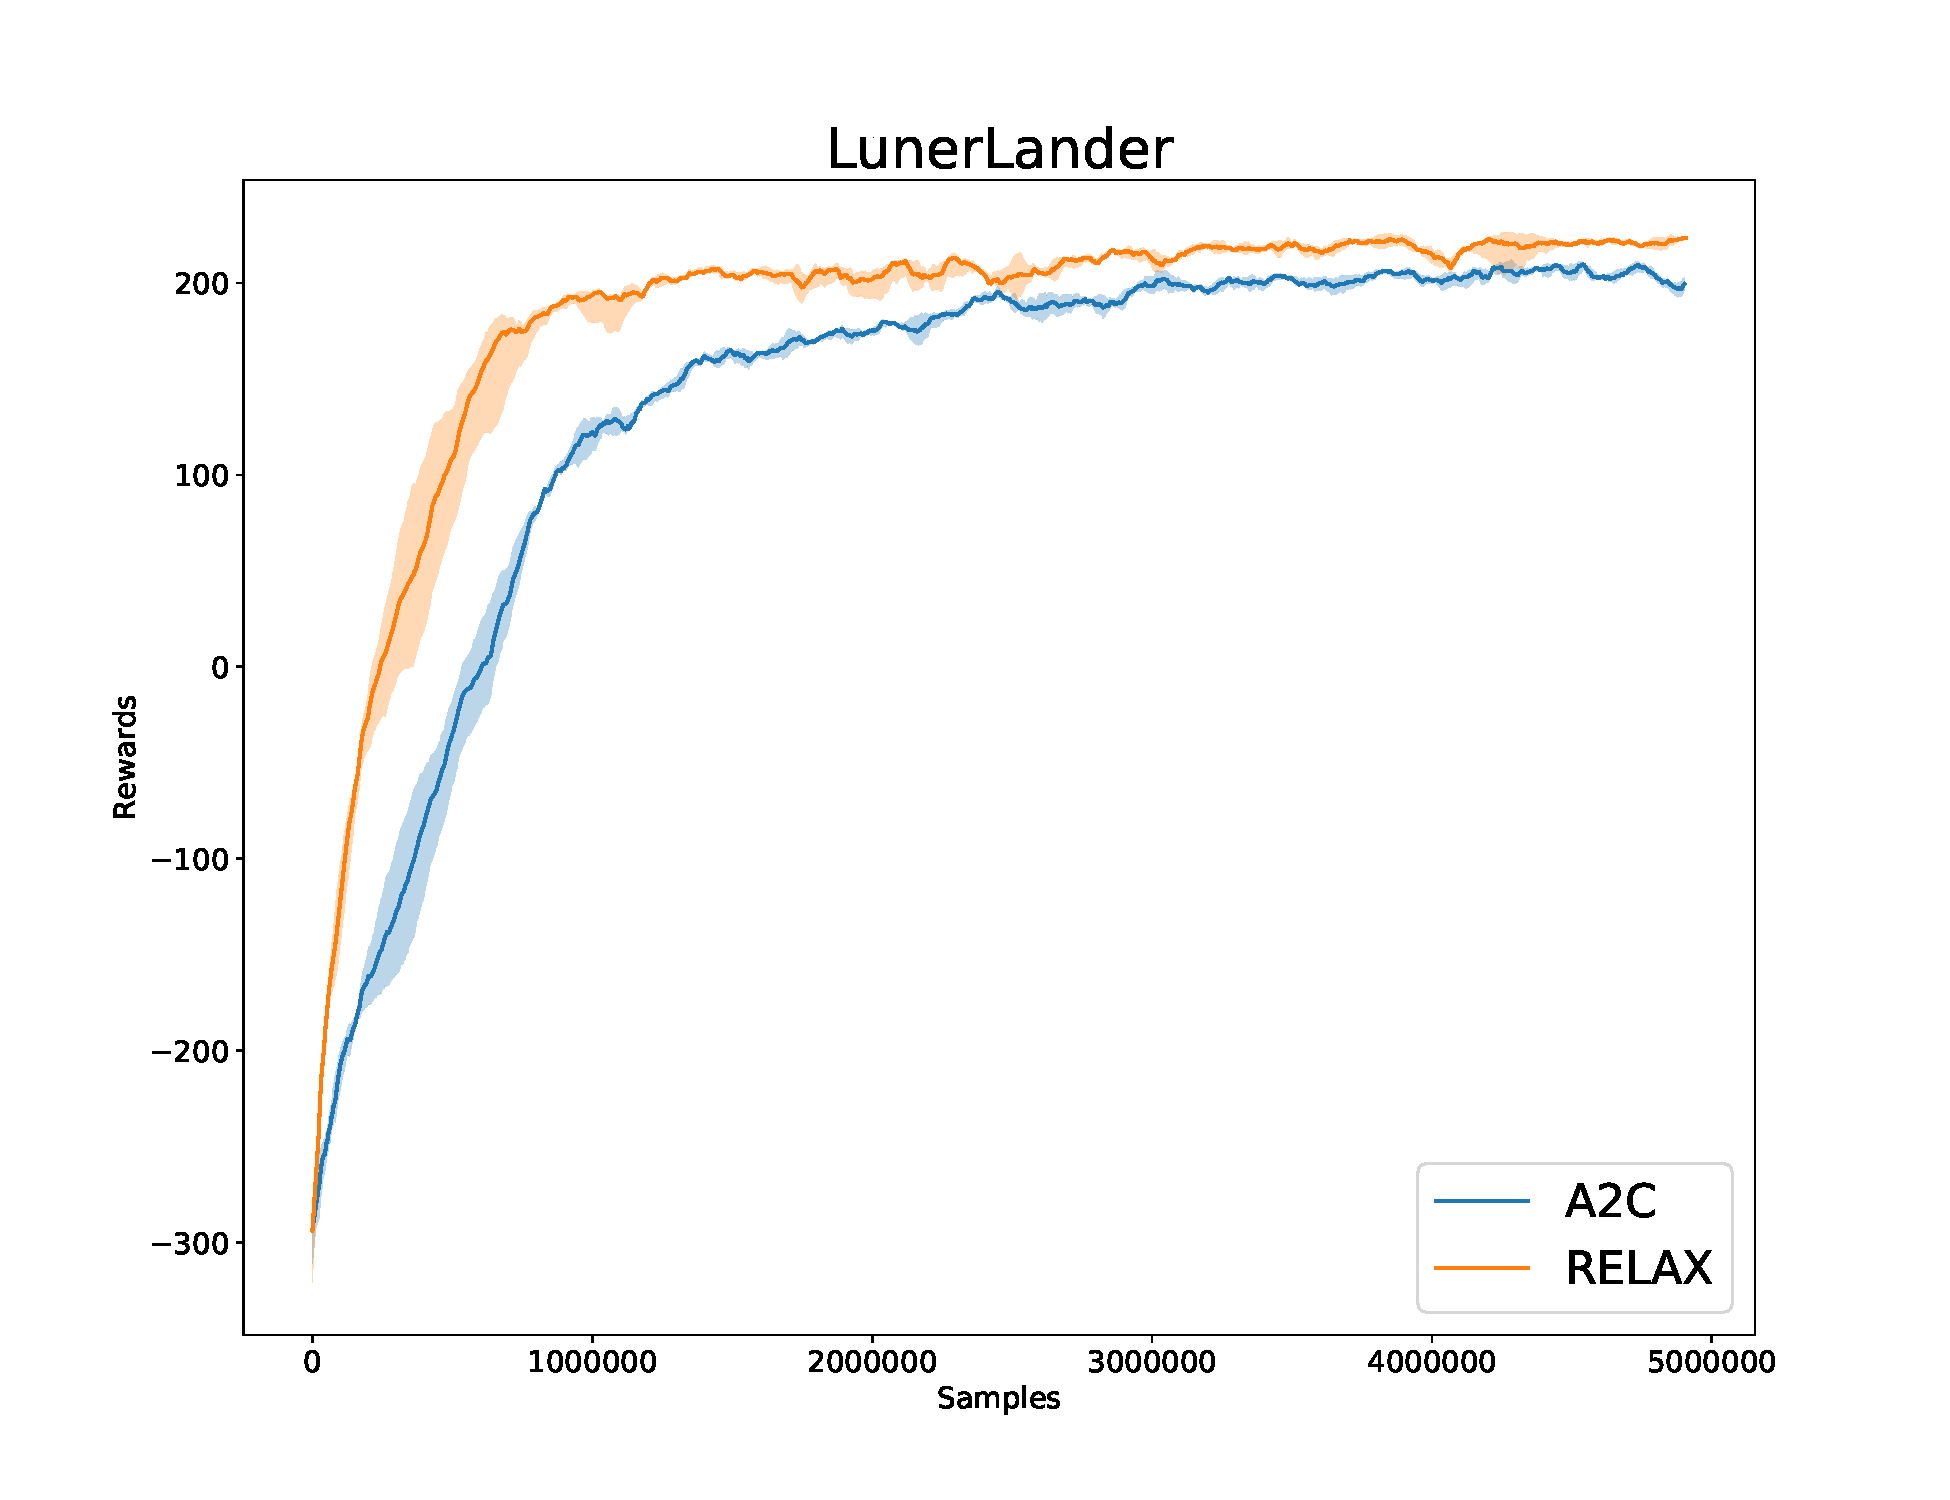
\includegraphics[width=.22\textwidth]{figures/ll_paper}
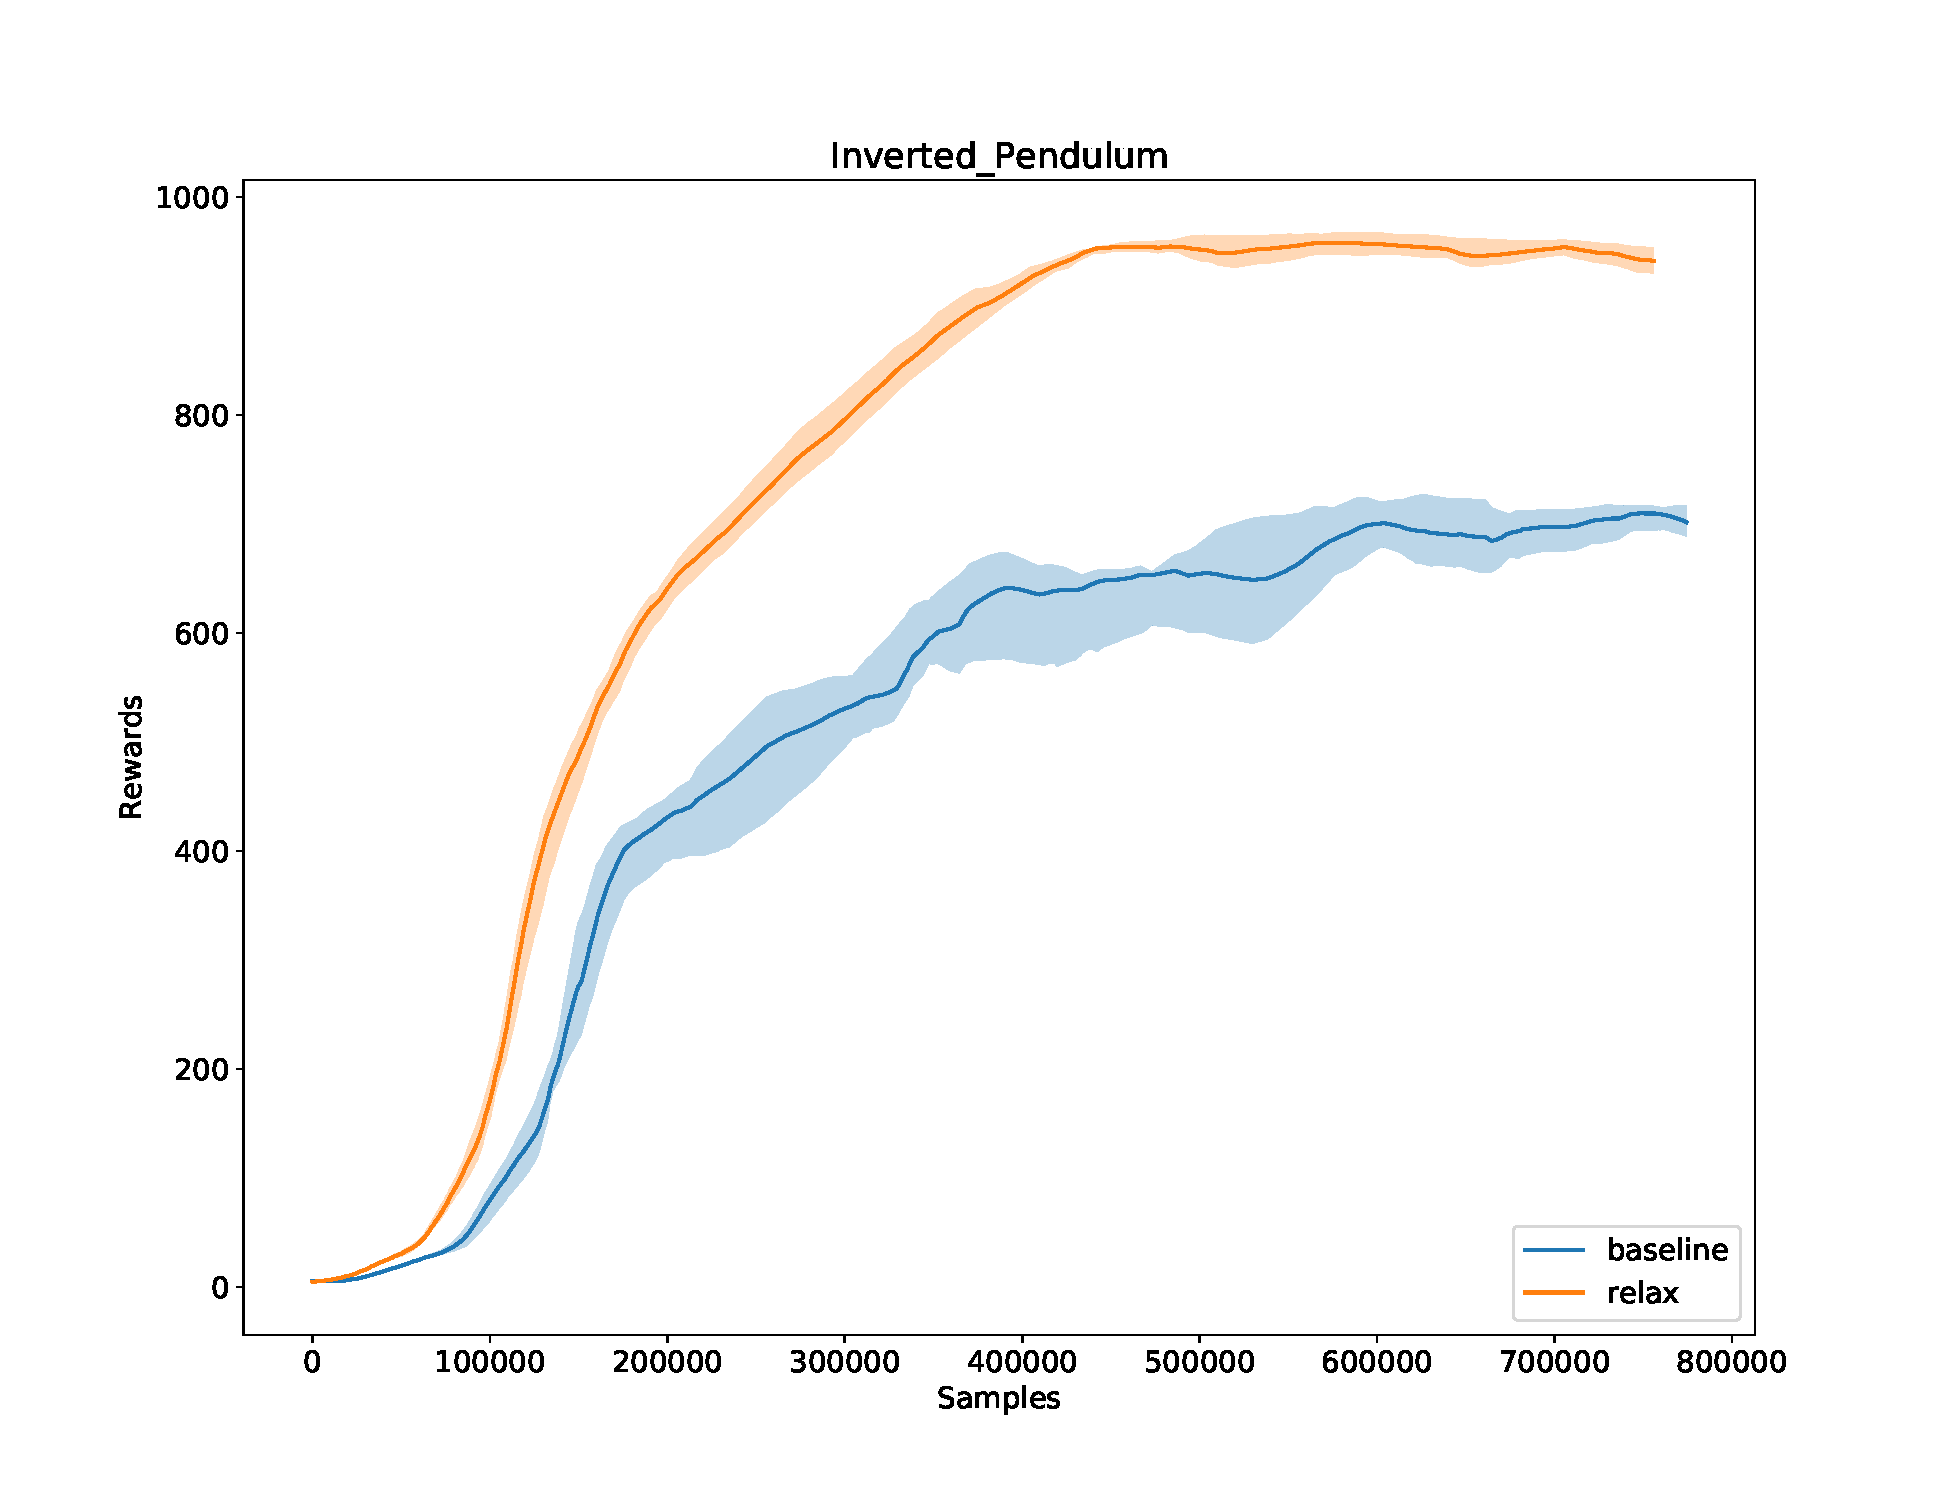
\includegraphics[width=.22\textwidth]{figures/Inverted_Pendulum_A2C}
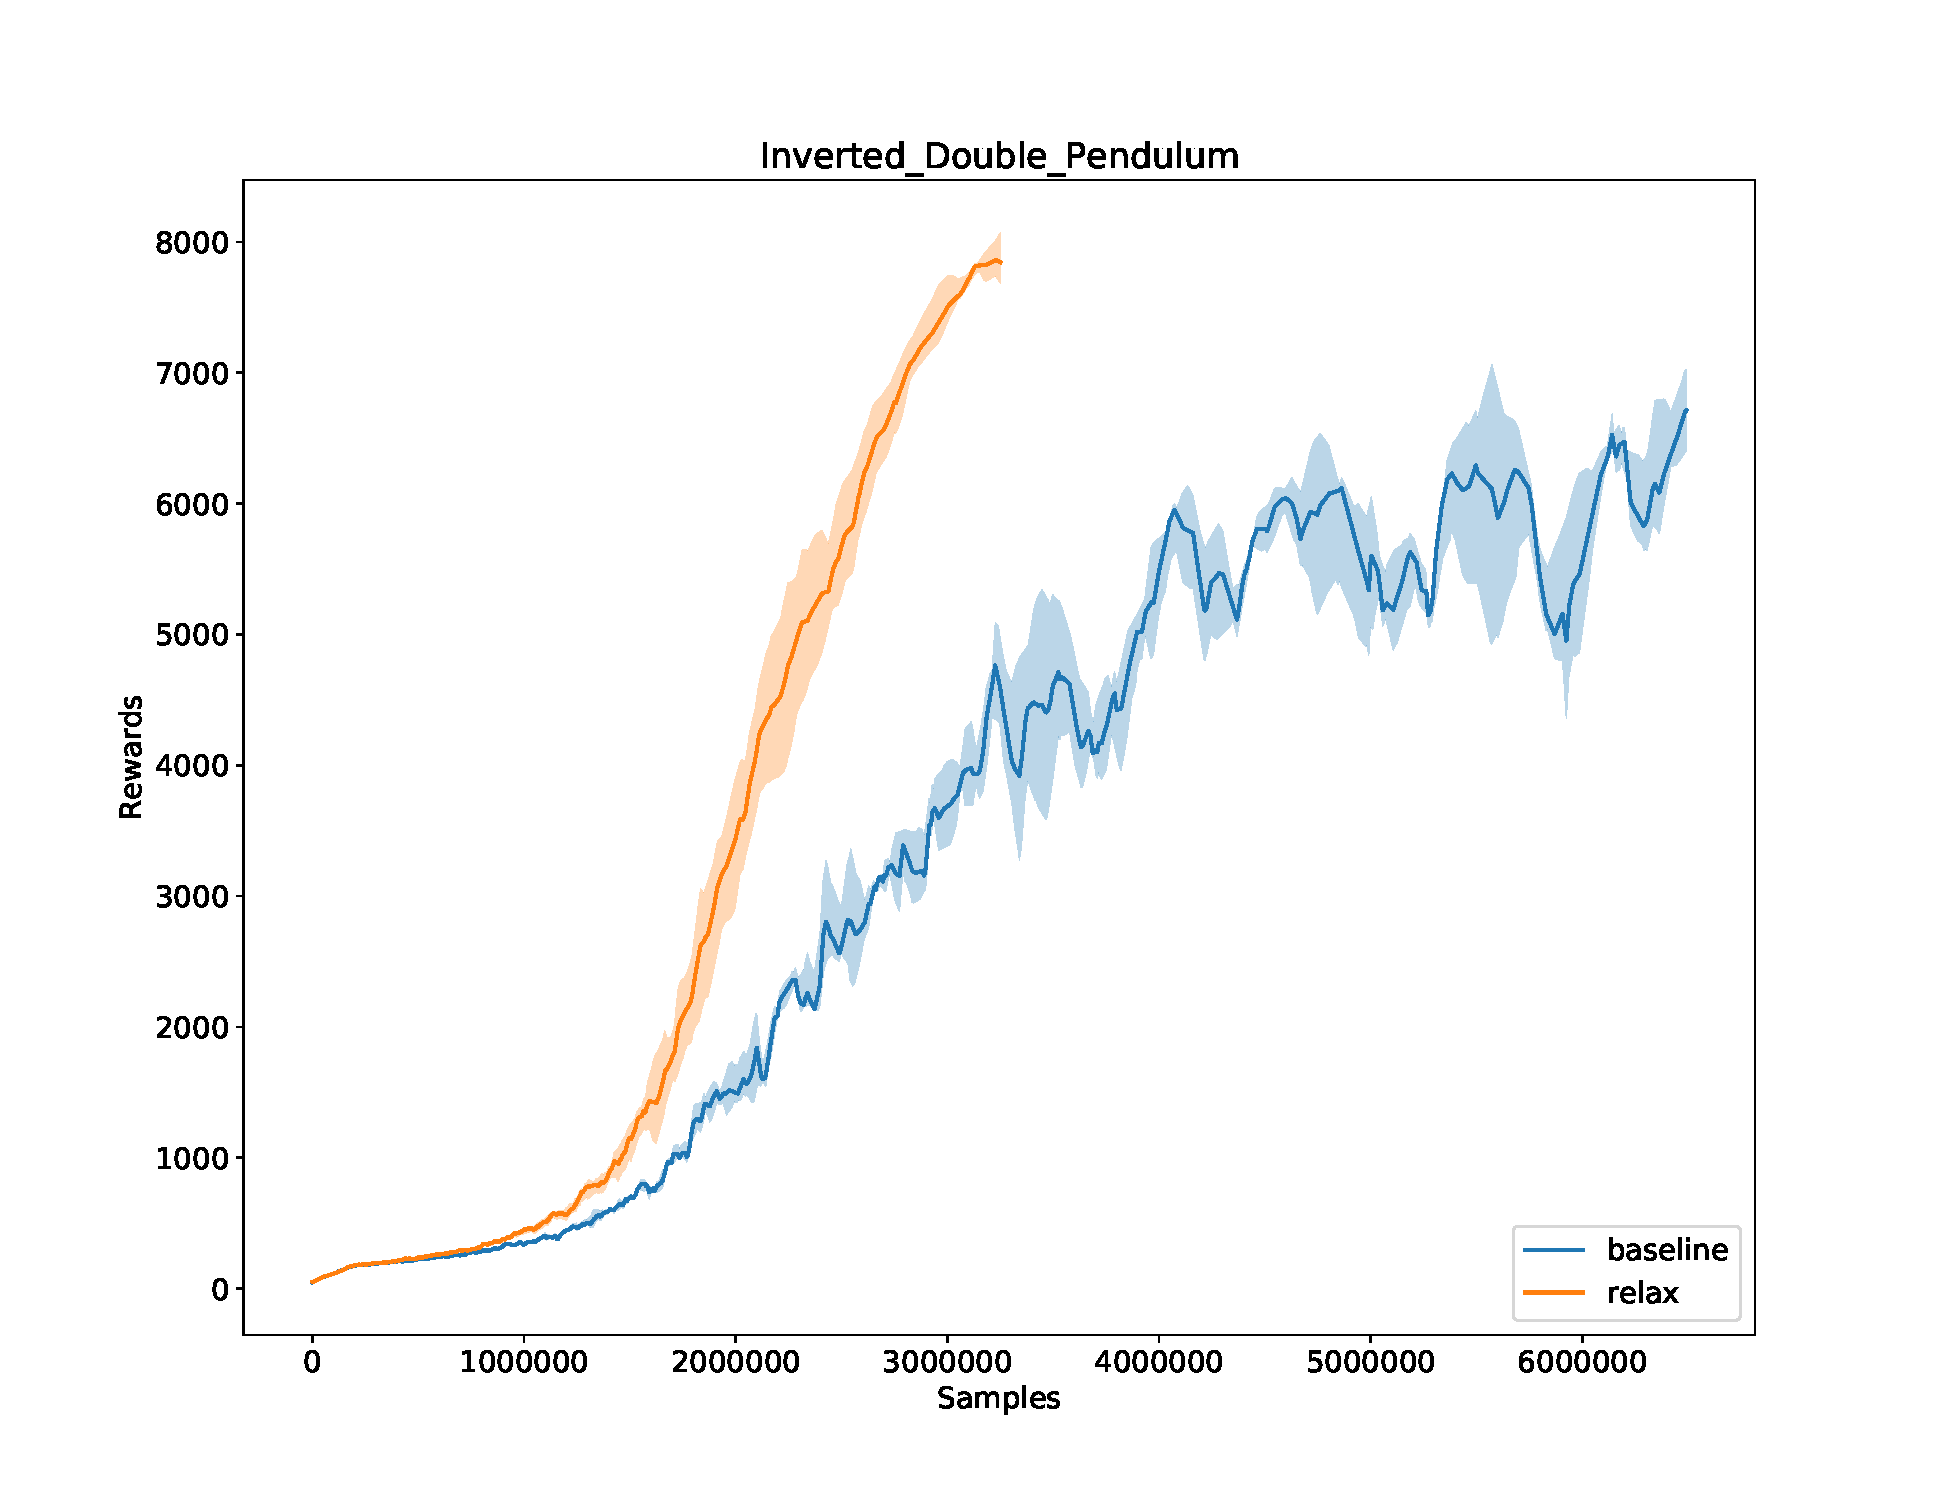
\includegraphics[width=.22\textwidth]{figures/Inverted_Double_Pendulum_A2C}
\caption{RL Experiments. Left to right: Cart Pole, Lunar Lander, Inverted Pendulum, Inverted Double Pendulum. In each curve, the center line indicates the mean reward over 5 random seeds. The opaque bars indicate the 25th and 75th percentiles. Our model is in orange and the baseline is in blue.}
\label{fig:disc_rl}
\end{figure}

%\begin{figure}[h]
%	\centering
%	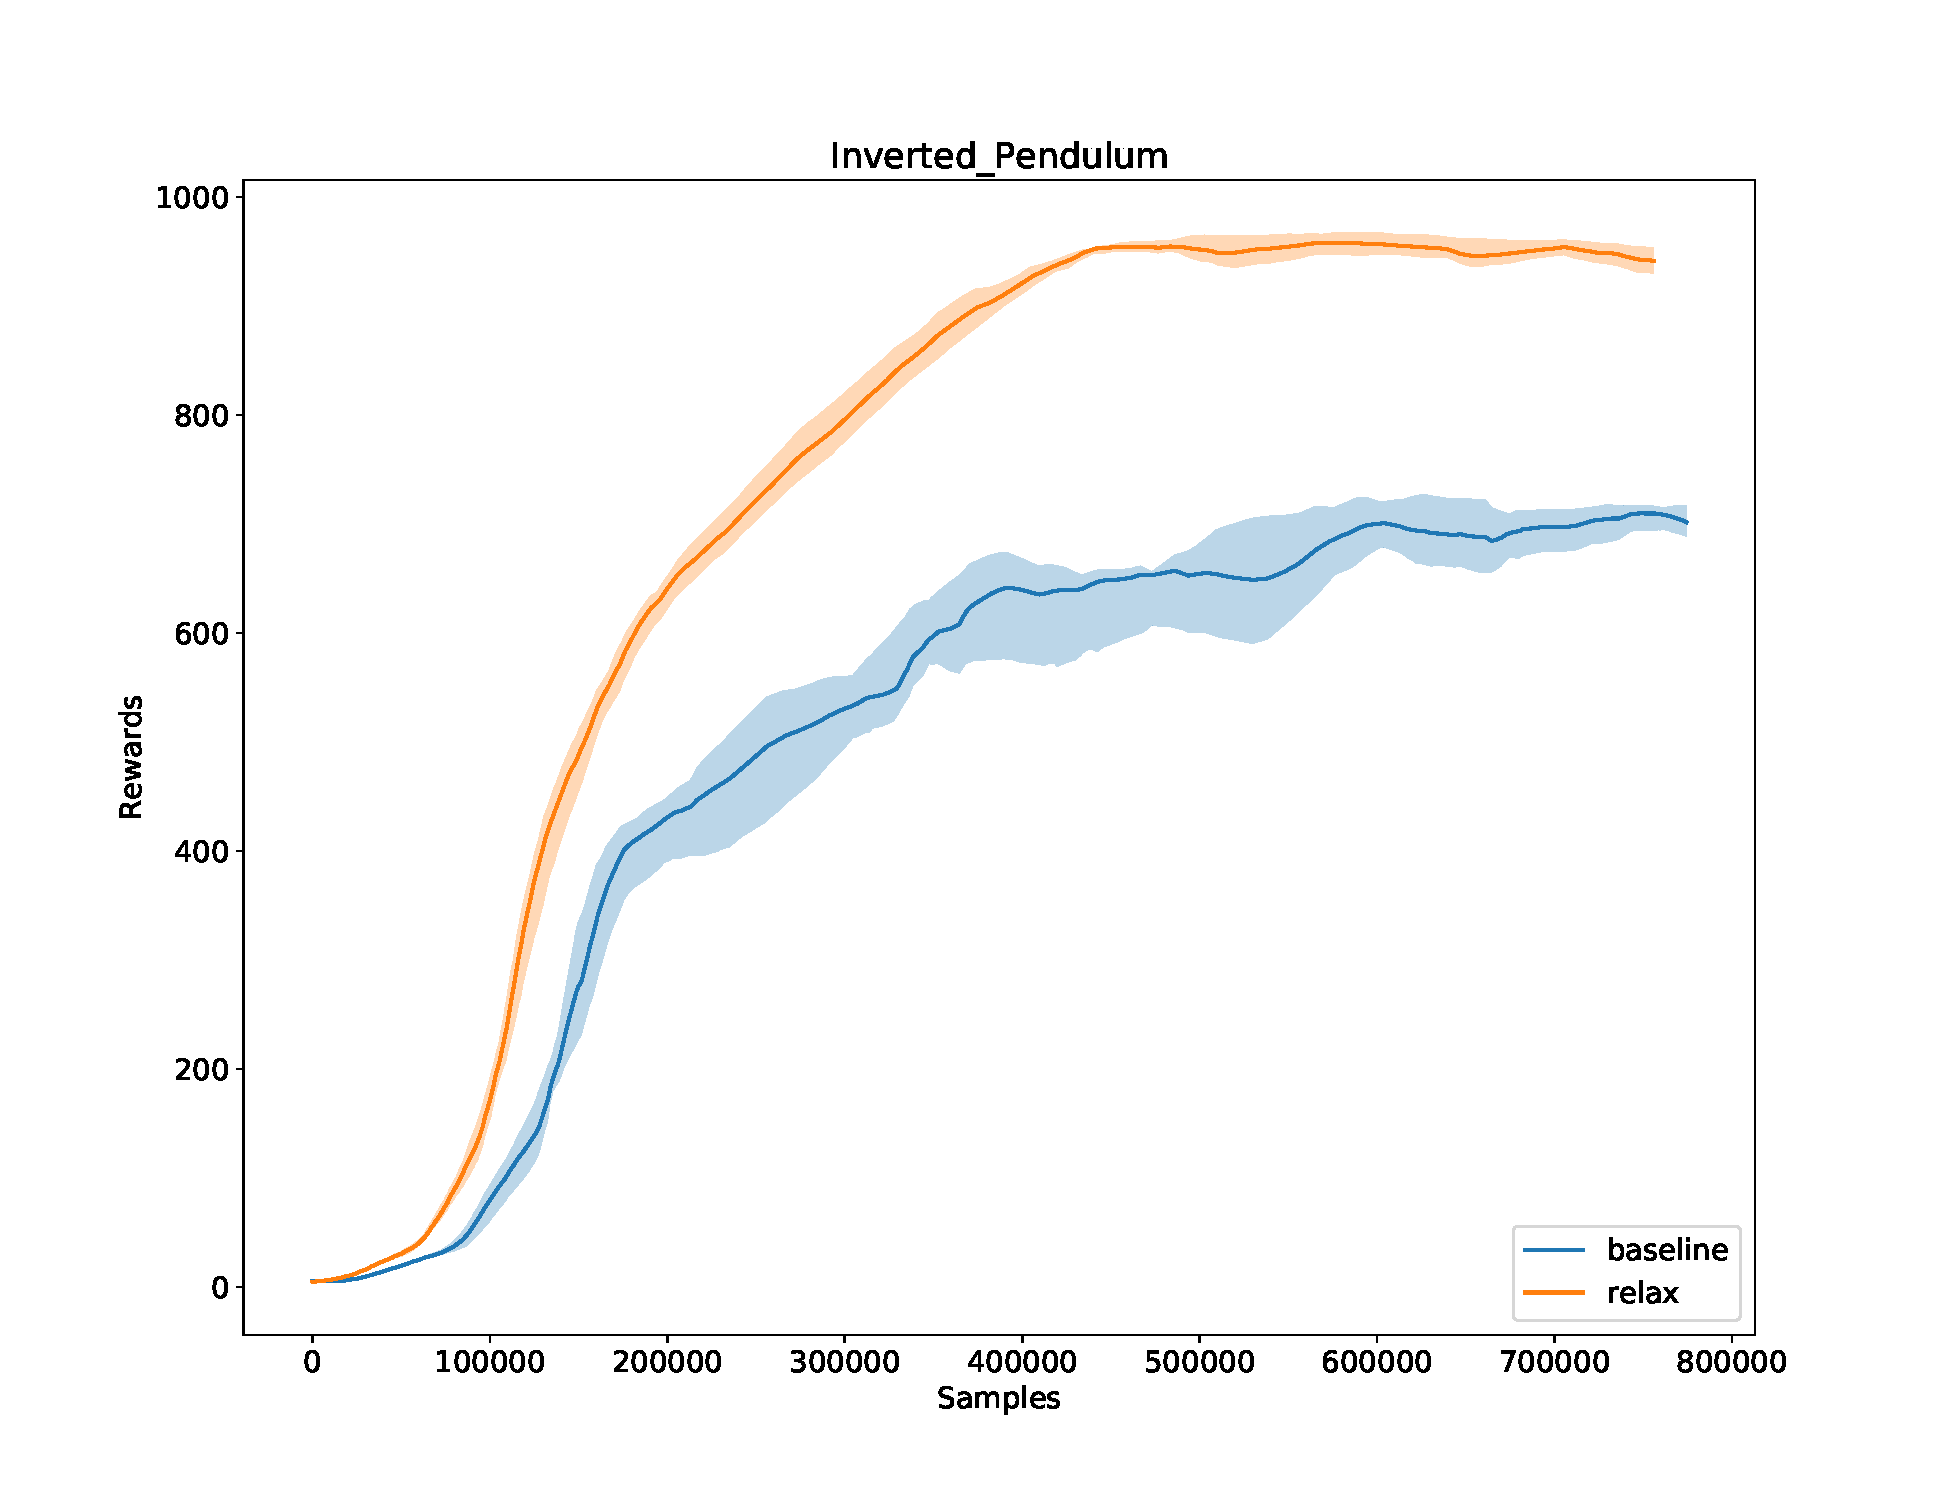
\includegraphics[width=.4\textwidth]{figures/Inverted_Pendulum_A2C}
%	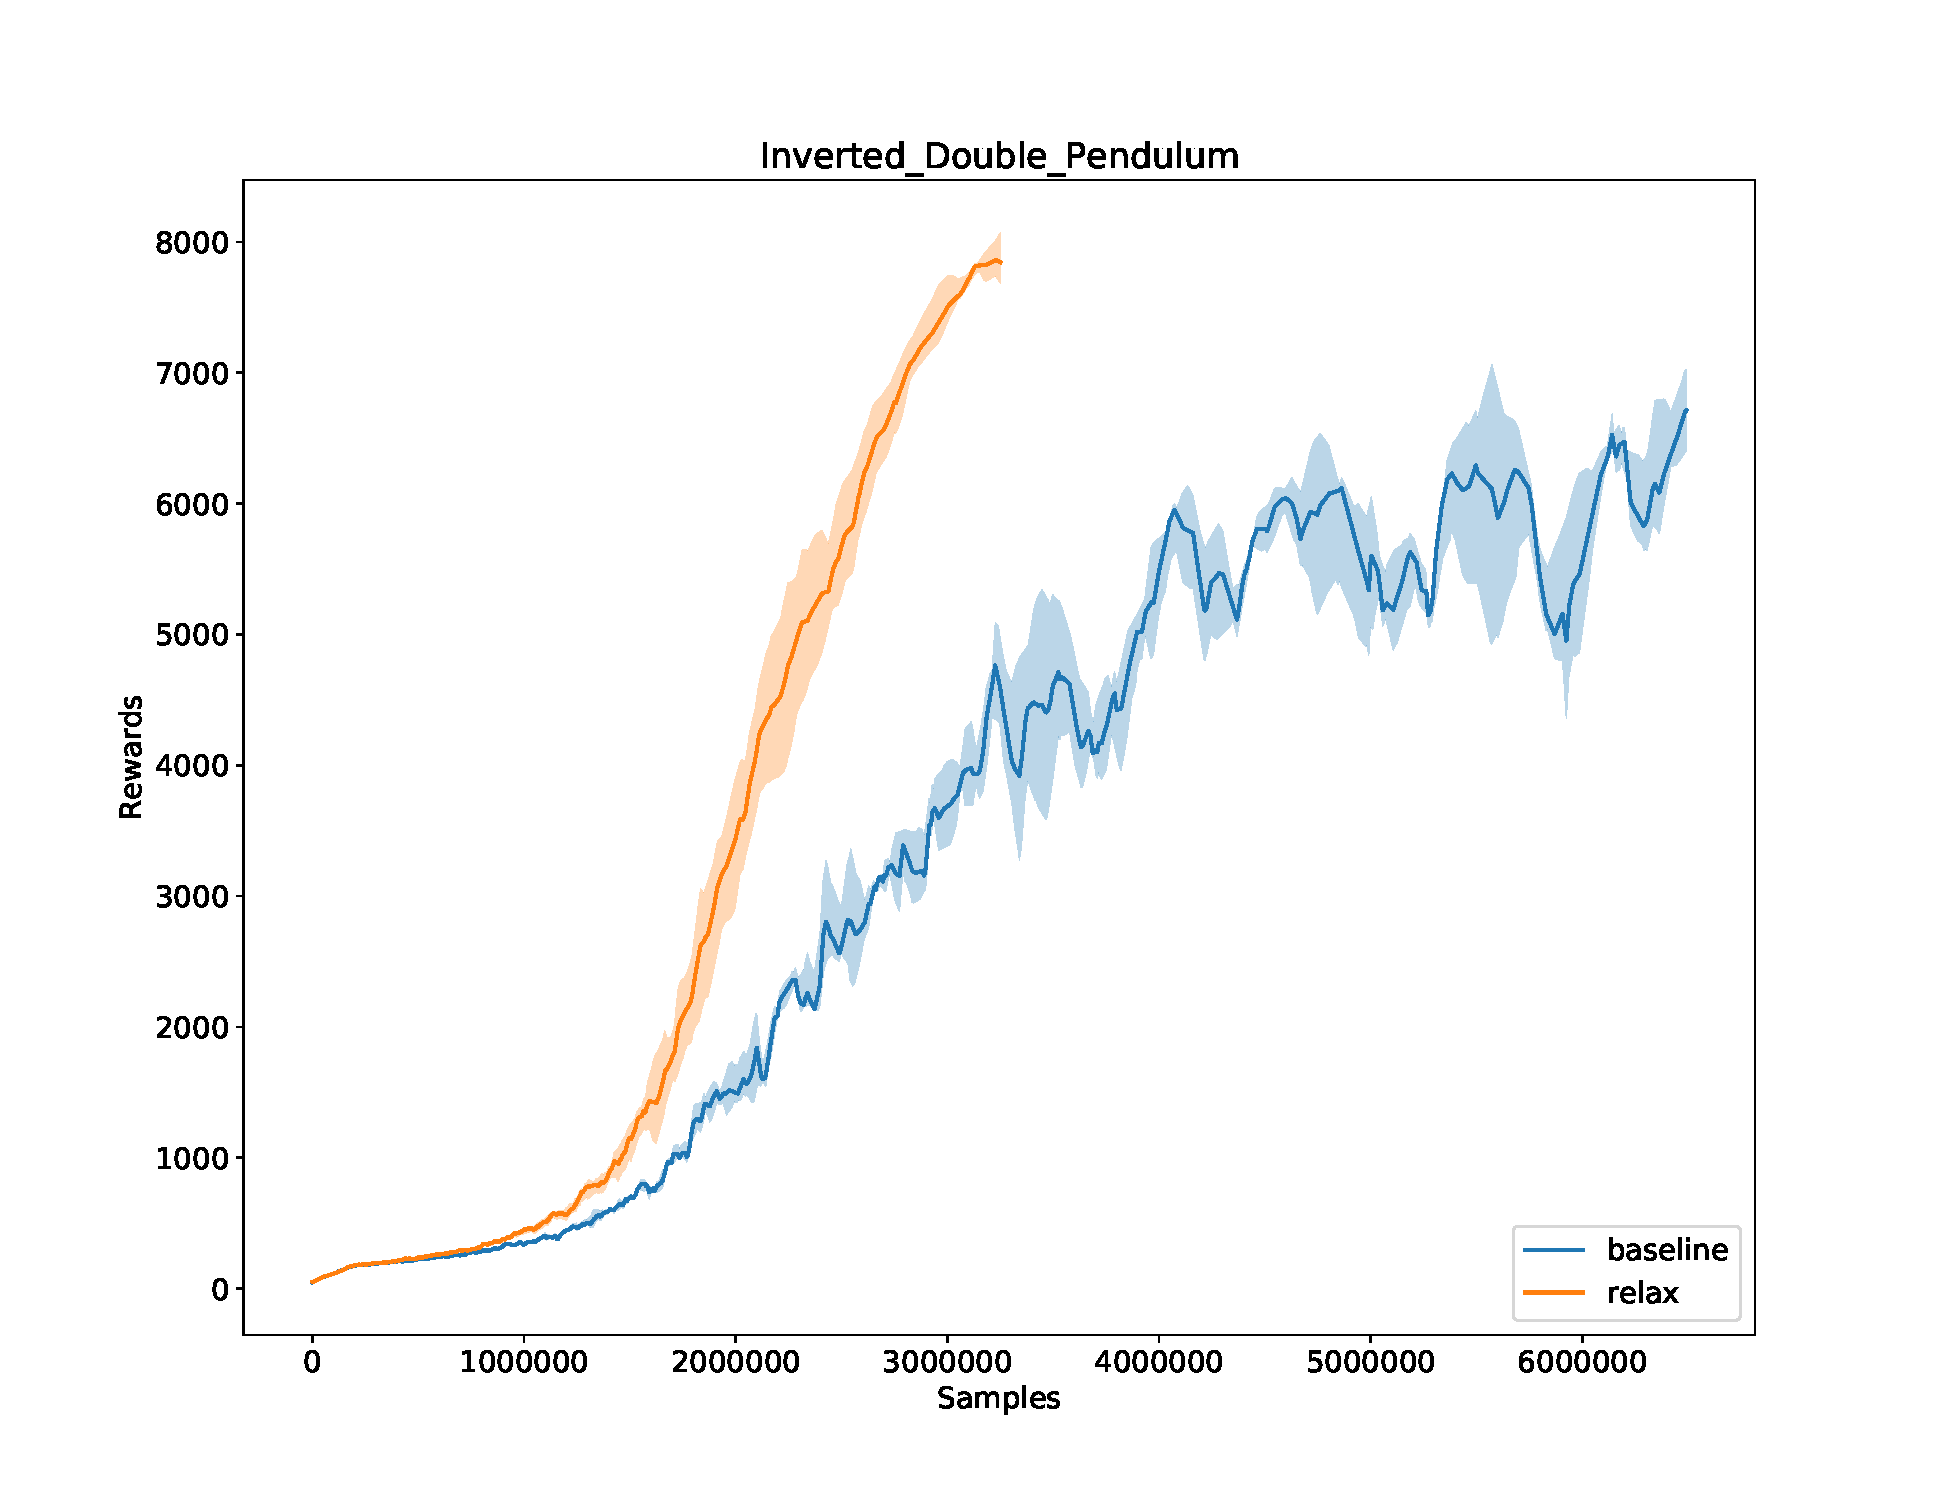
\includegraphics[width=.4\textwidth]{figures/Inverted_Double_Pendulum_A2C}
%	\caption{Continuous RL Experiments. \emph{Left:} Inverted Pendulum. \emph{Right:} Inverted Double Pendulum. In each curve, the center line indicates the mean reward over 5 random seeds. The opaque bars indicate the 25th and 75th percentiles.}
%	\label{fig:cont_rl}
%\end{figure}
% should i cut off the figure when relax stops training for the inverted double pendulum???


\section{Conclusions and future work}
\label{conclusion}

In this work, synthesized and generalized many of the standard approaches for constructing gradient estimators.
We proposed a simple and generic gradient estimator that can be applied to expectations of known or black-box functions of discrete or continuous random variables. We also derive a simple extension to apply our method to reinforcement learning in both discrete and continuous action domains. 
This approach is relatively simple to implement and adds minimal computational overhead. 

The foundation of our approach is the score function gradient estimator with a control variate whose expectation can be estimated with low variance using the reparameterization trick.
This control variate is neural network which is trained directly to minimize the variance of the estimated gradients.
The central result of this paper is that learning the function in the control variate leads to even better convergence properties and lower variance gradient estimates. 

The scope and generality of our estimator opens up many new possibilities for models which can now be trained via gradient decent. For example, we could apply our estimator to train a VAE with continuous latent variables who's generative model is non-differentiable (a rendering engine perhaps). We also feel that there is much room to explore model design choices for the control variate and develop a greater understand the properties of the optimal control variate. 

We believe our results in reinforcement learning are quite promising and should motivate further research into using action-dependent control-variates for policy-gradient methods. We are interested in combining our approach with other popular variance reduction techniques such as generalized advantage estimation \cite{kimura2000analysis}. We are also interested in ways to train our control variate off-policy as in $Q$-prop~\cite{gu2016q}. We also feel that the relationship between our learned control variate and the action-value function (commonly denoted as $Q$) is worth exploring and understanding in greater detail than we do now. 
Other possible applications:

%\section*{Acknowledgements}  % Uncomment for arxiv
%We thank Tian Qi Chen for helpful discussions.

\bibliography{bibliography}
\bibliographystyle{iclr2018_conference}




% ** Questions to answer: 
% (1) is z-tilde a clever way of using Rao-Blackwellization for a part of the reparameterization gradient? This would mean that the reparameterization z-tilde is related to the sufficient statistic of the estimator...
% (1) also maybe: the Q function has the opportunity to learn an estimator based on the sufficient statistics of the model, which by Rao-Blackwell-Kolmogorov is lower variance
% (2) What's a better notation to keep the dependence of z on $\theta$ in view?
% (3) is the REBAR control variate really using the reparameterization gradient in a meaningful way? Or, is it best viewed as just another f + control variate where control variate is cleverly designed with lower variance? 


%\par{Generalizing the reparameterization trick}

%Write sample from distribution $s(\epsilon)$ as $\epsilon = \mathcal{T}^{-1}(\mathbf{z}; \mathbf{\nu})$ for some invertible transform $\mathcal{T}$ with variational parameters $\nu$.
%write out transformed density
%example: normal with standard normal $s$
%example: inverse CDF of Gaussian with uniform $s$
%write out expected gradient under transformation
%show decomposition of expected gradient into reparameterization and correction terms 

%\par{Applying GRG to REBAR}

%show mapping of terms
%note denser derivation in REBAR appendix

%\par{Interpreting REBAR through GRG}

\clearpage
\section*{Appendices}
\appendix

\section{Conditional Re-sampling for Discrete Random Variables}
\label{resample}
When applying the RELAX estimator to a function of discrete random variables $b \sim p(b|\theta)$, we require that there exists a distribution $p(z|\theta)$ and a deterministic mapping $H(z)$ such that if $z \sim p(z|\theta)$ then $H(z) = b \sim p(b|\theta)$. Treating both $b$ and $z$ as random, this procedure defines a probabalistic model $p(b, z | \theta) = p(b|z)p(z|\theta)$. The RELAX estimator requires reparameterized samples from $p(z|\theta)$ and $p(z|b,\theta)$. We describe how to sample from these distributions in the common cases of $p(b|\theta) = \text{Bernoulli}(\theta)$ and $p(b|\theta) = \text{Categorical}(\theta)$.

\paragraph{Bernoulli} When $p(b|\theta)$ is Bernoulli distribution we let $H(z) = \mathbb{I}(z>0)$ and we sample from $p(z|\theta)$ with 
$$ z = \log \frac{\theta}{1 - \theta} + \log \frac{u}{1-u}, \qquad u \sim \text{uniform}[0,1].
$$ 
We can sample from $p(z|b, \theta)$ with 
\[
\tilde{z} =    \left\{
\begin{array}{ll}
      v\cdot\theta & b = 0 \\
      v(1-\theta) + \theta & b = 1 \\
\end{array} 
\right.
\]
where $v \sim \text{uniform}[0, 1]$.

\paragraph{Categorical} When $p(b|\theta)$ is a Categorical distribution where $\theta_i = p(b=i|\theta)$, we let $H(z) = \text{argmax}(z)$ and we sample from $p(z|\theta)$ with 
$$ z = \log\theta -\log(-\log u), \qquad u \sim \text{uniform}[0,1]^k
$$ where $k$ is the number of possible outcomes.

Intuitively, to sample from $p(z|b, \theta)$ we should first sample $v\sim \text{uniform}[0, 1]^k$, then compute $g_b = \log\theta_b -\log(-\log(v_b))$. Then we must determine how to scale each $v_{i\neq b}$ such that $g_{i\neq b} < g_b$. We can define $v'$ such that
\[
v_i' =    \left\{
\begin{array}{ll}
      v_i & i = b \\
      v_i\cdot(v_b)^{\frac{\theta_i}{\theta_b}} & i \neq b \\
\end{array} 
\right.
\] and then $\tilde{z} = \log\theta - \log(-\log v')$ which is our sample from $p(z|b, \theta)$. 

%Let $G_{1:k} = -\log-\log(U_{i:k})$ be samples from the Gumbel distribution, and learnable parameters $(\alpha_1, \dots, \alpha_k)$ be interpreted as some unnormalized parameterization of the discrete distribution under consideration.
%Then, consider the following sampling procedure: for each k, find the k that maximizes $\log \alpha_k - G_k$, and then set $D_k=1$ and $D_{i \neq k} = 0$. The Gumbel-Max trick states that sampling from the discrete distribution is equivalent to taking this argmax, that is, $p(D_k = 1) = \alpha_k / \sum_{i=1}^n \alpha_i$.

%Since taking an argmax is still a discontinuous operation, \cite{maddison2016concrete} and \cite{jang2016categorical} proposed further relaxing the argmax operator through the softmax function with an additional temperature parameter $\lambda$:
%\begin{equation}
%x_k = \frac{\exp\{( \log \alpha_k+ G_k) / \lambda\}}{\sum_{i=1}^n\exp\{( \log \alpha_i+ G_i) / \lambda\}}
%\end{equation}
%This relaxation allows values within the simplex, but in the low temperature limit, it becomes exactly the discrete argmax.
%One limitation of the concrete distribution is that it is a biased estimator except in limiting temperature.
%In other words, a small amount of bias is present for a non-zero temperature.



\section{Derivations of estimators used in Reinforcement learning}
\label{rl appendix}
We give the derivation of the \LAX{} estimator used for continuous RL tasks.
\begin{theorem}
The \LAX{} estimator,
\begin{align}
\hat g_\LAX^{\RL} = \sum_{t=1}^{\infty} \LL{t} \left[ \sum_{t'=t}^{\infty} r_{t'} - c_\phi(a_t,s_t) \right] +\frac{\partial}{\partial\theta} c_\phi(a_t, s_t), \\
a_t = a_t(\epsilon_t,s_t,\theta), \quad \epsilon_t \sim p(\epsilon_t)\nonumber,
\end{align}
is unbiased.
\end{theorem}
\begin{proof}
Note that by using the score-function estimator, for all $t$, we have 
%
\begin{align*}
\E_{p(\tau)}\Big[\LL{t} c_\phi(a_t, s_t)\Big] = \E_{p(a_{1:t-1},s_{1:t})}\Big[\frac{\partial}{\partial\theta}\E_{\pi(a_t|s_t, \theta)}\Big[c_\phi(a_t, s_t)\Big]\Big].
\end{align*}
Then, by adding and subtracting the same term, we have
\begin{align*}
\PT\E_{p(\tau)}[f(\tau)] &= \E_{p(\tau)}\left[f(\tau)\cdot\LP{\tau;\theta}\right]-\sum_t\E_{p(\tau)}\Big[\LL{t} c_\phi(a_t, s_t)\Big]+\\&\sum_t \E_{p(a_{1:t-1},s_{1:t})}\Big[\frac{\partial}{\partial\theta}\E_{\pi(a_t|s_t, \theta)}\Big[c_\phi(a_t,s_t)\Big]\Big]\nonumber\\
&= \E_{p(\tau)}\left[ \sum_{t=1}^{\infty} \LL{t}\left(\sum_{t'=t}^{\infty} r_{t'} - c_\phi(a_t,s_t)\right)\right]+\sum_t \E_{p(a_{1:t-1},s_{1:t})}\Big[\E_{p(\epsilon_t)}\Big[\frac{\partial}{\partial\theta}c_\phi(a_t(\epsilon_t,s_t,\theta), s_t)\Big]\Big]\nonumber\\
&= \E_{p(\tau)}\left[ \sum_{t=1}^{\infty} \LL{t}\left(\sum_{t'=t}^{\infty} r_{t'} - c_\phi(a_t,s_t)\right)+\frac{\partial}{\partial\theta}c_\phi(a_t(\epsilon_t,s_t,\theta), s_t)\right]\nonumber
\end{align*}
\end{proof}

In the discrete control setting, our policy parameterizes a soft-max distribution which we use to sample actions. We define $z_t\sim p(z_t|s_t)$, which is equal to $\sigma (\log\pi - \log(-\log(u)))$ where $u\sim \text{Unif}[0, 1]$, $a_t = \text{argmax}(z_t)$, $\sigma$ is the soft-max function. We also define $\tilde{z_t} \sim p(z_t|a_t,s_t)$ and uses the same reparametrization trick for sampling $\tilde{z_t}$ as explicated in Appendix \ref{resample}.
\begin{theorem}
The \RELAX{} estimator,
\begin{align}
\hat g_\RELAX^{\RL} = \sum_{t=1}^{\infty} \LL{t}\left(\sum_{t'=t}^{\infty} r_{t'} - c_\phi(\tilde{z}_t, s_t)\right)-\frac{\partial}{\partial\theta}c_\phi(\tilde{z}_t, s_t)+\frac{\partial}{\partial\theta}c_\phi(z_t, s_t), \label{eq:relaxrlproof}\\
\tilde{z}_t \sim p(z_t|a_t,s_t), \qquad z_t \sim p(z_t|s_t)\nonumber, 
\end{align}
is unbiased.
\end{theorem}
\begin{proof}
Note that by using the score-function estimator, for all $t$, we have 
%
\begin{align*}
\E_{p(a_{1:t},s_{1:t})}\Big[\LL{t} \E_{p(z_t|a_t,s_t)}[c_\phi(z_t, s_t)]\Big] &= \E_{p(a_{1:t-1},s_{1:t})}\Big[\frac{\partial}{\partial\theta}\E_{\pi(a_t|s_t, \theta)}\Big[\E_{p(z_t|a_t,s_t)}[c_\phi(z_t, s_t)]\Big]\Big]\\
&=\E_{p(a_{1:t-1},s_{1:t})}\Big[\frac{\partial}{\partial\theta}\E_{p(z_t|s_t)}[c_\phi(z_t, s_t)]\Big]
\end{align*}
Then, by adding and subtracting the same term, we have
\begin{align*}
\PT\E_{p(\tau)}[f(\tau)] &= \E_{p(\tau)}\left[f(\tau)\cdot\LP{\tau;\theta}\right]-\sum_t\E_{p(a_{1:t},s_{1:t})}\Big[\LL{t} \E_{p(z_t|a_t,s_t)}[c_\phi(z_t, s_t)]\Big]+\\
&\sum_t\E_{p(a_{1:t-1},s_{1:t})}\Big[\frac{\partial}{\partial\theta}\E_{p(z_t|s_t)}[c_\phi(z_t, s_t)]\Big]\nonumber\\
&= \E_{p(\tau)}\left[ \sum_{t=1}^{\infty} \LL{t}\left(\sum_{t'=t}^{\infty} r_{t'} - \E_{p(z_t|a_t,s_t)}[c_\phi(z_t, s_t)]\right)\right]\\&+\sum_t\E_{p(a_{1:t-1},s_{1:t})}\Big[\frac{\partial}{\partial\theta}\E_{p(z_t|s_t)}[c_\phi(z_t, s_t)]\Big]\nonumber\\
&= \E_{p(\tau)}\Big[ \sum_{t=1}^{\infty} \LL{t}\left(\sum_{t'=t}^{\infty} r_{t'} - \E_{p(z_t|a_t,s_t)}[c_\phi(z_t, s_t)\right)\\
&-\frac{\partial}{\partial\theta}\E_{p(z_t|a_t,s_t)}[c_\phi(z_t, s_t)]+\frac{\partial}{\partial\theta}\E_{p(z_t|s_t)}[c_\phi(z_t, s_t)]\Big]\nonumber
\end{align*}
Since $p(z_t|s_t)$ is reparametrizable, we obtain the estimator in Eq.(\ref{eq:relaxrlproof}).
\end{proof}




\section{Experimental Details}
\label{experiment appendix}

\subsection{Discrete VAE}
\label{app_disc_vae}
In the one layer models we optimize the evidence lower bound (ELBO): $$\log p(x) \geq \mathcal{L}(\theta) = \E_{q(b|x)}[\log p(x|b) + \log p(b) - \log q(b|x)]$$ where $q(b_1|x) = \sigma(x\cdot W_q + \beta_q)$ and $p(x| b_1) = \sigma(b_1\cdot W_p + \beta_p)$ with weight matrices $W_q,W_p$ and bias vectors $\beta_q,\beta_p$.
The parameters of the prior $p(b)$ are also learned.

We run all models for $2,000,000$ iterations with a batch size of $24$. For the REBAR models, we tested learning rates in $\{.005, .001, .0005,  .0001, .00005\}$. 

RELAX adds more hyperparameters.
These are the depth of the neural network component of our control variate $r_\rho$, the weight decay placed on the network, and the scaling on the learning rate for the control variate.
We tested neural network models with $l$ layers of 200 units using the ReLU nonlinearity with $l \in \{2, 4\}$.
We trained the control variate with weight decay in $\{.001, .0001\}$. We trained the control variate with learning rate scaling in $\{1, 10\}$.

To limit the size of hyperparameter search for the RELAX models, we only test the best performing learning rate for the REBAR baseline and the next largest learning rate in our search set.
In many cases, we found that RELAX allowed our model to converge at learning rates which made the REBAR estimators diverge.
We believe further improvement could be achieved by tuning this parameter.

All presented results are from the models which achieve the highest ELBO on the validation data.

\subsubsection{Two layer model}
In the two layer models we optimize the ELBO $$\mathcal{L}(\theta) = \E_{q(b_2|b_1)q(b_1|x)}[\log p(x|b_1) + \log p(b_1|b_2) + \log p(b_2) - \log q(b_1|x) - \log q(b_2|b_1)]$$ where $q(b_1|x) = \sigma(x\cdot W_{q_1} + \beta_{q_1})$, $q(b_2|b_1) = \sigma(b_1\cdot W_{q_2} + \beta_{q_2})$, $p(x| b_1) = \sigma(b_1\cdot W_{p_1} + \beta_{p_1})$, and $p(b_1| b_2) = \sigma(b_2\cdot W_{p_2} + \beta_{p_2})$ with weight matrices $W_{q_1},W_{q_2},W_{p_1},W_{p_2}$ and biases $\beta_{q_1},\beta_{q_2},\beta_{p_1},\beta_{p_2}$. As in the one layer model, the prior $p(b_2)$ is also learned.

We run an identical hyperpameter search in the 2 layer model as we do in the 1 layer model. 


\subsection{Discrete RL}
In both the baseline A2C and RELAX models, the policy and control variate (value function in the baseline model) were 2 layer neural networks with 10 units per layer. The ReLU non linearity was used on all layers except for the output layer.

For these tasks we estimate the policy gradient with a single monte-carlo sample. We run one episode of the environment to completion, compute the discounted rewards, and run one iteration of gradient decent. We believe using larger batches will improve performance but would less clearly demonstrate the potential of our method. 

As our control variate does not have the same interpretation as the value function of A2C, it was not directly clear how to add reward bootstrapping and other variance reduction techniques common in RL into our model. We leave the task of incorporating these and other variance reduction techniques to future work.  

Both models were trained with the RMSProp \cite{Tieleman2012} optimizer and a reward discount factor of $.99$ was used.

Both models have 2 hyperparameters to tune; the global learning rate and the scaling factor on the learning rate for the control variate (or value function). We complete a grid search for both parameters in $\{0.01, 0.003, 0.001\}$ and present the model which ``solves'' the task in the fewest number of episodes averaged over 5 random seeds. ``Solving'' the tasks was defined by the creators of the OpenAI gym \cite{1606.01540}. The Cart Pole task is considered solved if the agent receives an average reward greater than 195 over 100 consecutive episodes. The Lunar Lander task is considered solved if the agent receives an average reward greater than 200 over 100 consecutive epsidoes. 

The Cart Pole experiments were run for 250,000 frames. The Lunar Lander experiments were run for 5,000,000 frames. 

\subsection{Continuous RL}
The continuous tasks uses both the value function and the control variate to enable bootstrapping, which is needed due to the increased complexity of the problem. Our model architecture is base on OpenAI's baseline\cite{?} code for ACKTR\cite{?}. The three models- policy, value, and control variate, are 2 layer neural networks with 64 hidden units per layer. The value and control variate networks are identical, with the ELU nonlinearity in each hidden layer. The policy network has Tanh nonlinearity. The policy network, which parameterizes the gaussian policy comprises of a network (with the architecture mentioned above) that outputs the mean, and a separate, trainable log standard deviation value that is not input dependent. All three networks have a linear output layer. We selected the batch size to be 2500, meaning for a fixed timestep (2500) we collect multiple rollouts of a task and update the networks' parameters with the batch of episodes. Per one policy update, we optimize both the value and control variate network multiple times. The number of times we train  the value network is fixed to 25, while for the control variate, it was chosen to be a hyperparameter. 
%need to add information on whether we build on top of reinforce, or a2c or a2c+GAE
All models were trained, each with a separate ADAM \cite{kingma2015adam} otimizer, with $\beta_1=0.9$, $\beta_2=0.999$, and $\epsilon=1e-08$. 

The baseline A2C case has 2 hyperparameters to tune: the learning rate for the optimizer for the policy and value network. A grid search was done over the set: $\{0.03, 0.003, 0.003\}$. \RELAX has 4 hyperparameters to tune: 3 learning rates for the optimizer per network, and the number of training iterations of the control variate per policy gradient update. Due to the large number of hyperparameters, we restricted the size of the grid search set to $\{0.003, 0.0003\}$ for the learning rates, and $\{5, 25, 50\}$ for the control variate training iteration number. We picked the hyperparameter setting that yielded the shortest episode-to-completion time. As with the discrete case, we used the definition of completion defined by OpenAI gym\cite{1606.01540} for each task. 

The Inverted Pendulum experiments were run for 1,000,000 frames. The Inverted Double Pendulum experiments were run for 10,000,000 frames.

\end{document}

%For all models, the policy and control variate were both neural networks with 2 layers of 10 units using the ReLU nonlinearity.
%We first tuned the learning rate using the baseline A2C then ran \RELAX{} with the same learning rate. 
%Again, we are aware that improved results could be obtained by further tuning the learning rate for \RELAX{} but we wanted to illustrate the improvement provided solely by the improved control variate. 

%\paragraph{Experimental details}
%We estimate the policy gradient using a single Monte Carlo sample produced from a one episode roll-out of the current policy.
%We note that improved performance could be achieved by using more samples, but we intended to test our model in the highest-possible variance setting. 
%In all experiments both the policy and control variate were two layer neural networks with RELU non-linearities. Each intermediate layer's output had dimension 10.
%We searched over two hyper-parameters; the global learning rate and the scaling on the loss from the control variate or value function.
%For each we tested values in $[.01, .003, .001]$.
%Between our model and the baseline and the learning rates were also constant across tests making it that all improvements derive from having a lower variance estimate of the policy gradient.
%Presented results are obtained by averaging over 5 runs with different random seeds. We run the CartPole and LunarLander for $250,000$ and $5,000,000$ time-steps respectively. 